% Options for packages loaded elsewhere
\PassOptionsToPackage{unicode}{hyperref}
\PassOptionsToPackage{hyphens}{url}
%
\documentclass[
]{book}
\usepackage{amsmath,amssymb}
\usepackage{lmodern}
\usepackage{iftex}
\ifPDFTeX
  \usepackage[T1]{fontenc}
  \usepackage[utf8]{inputenc}
  \usepackage{textcomp} % provide euro and other symbols
\else % if luatex or xetex
  \usepackage{unicode-math}
  \defaultfontfeatures{Scale=MatchLowercase}
  \defaultfontfeatures[\rmfamily]{Ligatures=TeX,Scale=1}
\fi
% Use upquote if available, for straight quotes in verbatim environments
\IfFileExists{upquote.sty}{\usepackage{upquote}}{}
\IfFileExists{microtype.sty}{% use microtype if available
  \usepackage[]{microtype}
  \UseMicrotypeSet[protrusion]{basicmath} % disable protrusion for tt fonts
}{}
\makeatletter
\@ifundefined{KOMAClassName}{% if non-KOMA class
  \IfFileExists{parskip.sty}{%
    \usepackage{parskip}
  }{% else
    \setlength{\parindent}{0pt}
    \setlength{\parskip}{6pt plus 2pt minus 1pt}}
}{% if KOMA class
  \KOMAoptions{parskip=half}}
\makeatother
\usepackage{xcolor}
\IfFileExists{xurl.sty}{\usepackage{xurl}}{} % add URL line breaks if available
\IfFileExists{bookmark.sty}{\usepackage{bookmark}}{\usepackage{hyperref}}
\hypersetup{
  pdftitle={Mozambique National Adaptation Plan},
  pdfauthor={The A Team},
  hidelinks,
  pdfcreator={LaTeX via pandoc}}
\urlstyle{same} % disable monospaced font for URLs
\usepackage{longtable,booktabs,array}
\usepackage{calc} % for calculating minipage widths
% Correct order of tables after \paragraph or \subparagraph
\usepackage{etoolbox}
\makeatletter
\patchcmd\longtable{\par}{\if@noskipsec\mbox{}\fi\par}{}{}
\makeatother
% Allow footnotes in longtable head/foot
\IfFileExists{footnotehyper.sty}{\usepackage{footnotehyper}}{\usepackage{footnote}}
\makesavenoteenv{longtable}
\usepackage{graphicx}
\makeatletter
\def\maxwidth{\ifdim\Gin@nat@width>\linewidth\linewidth\else\Gin@nat@width\fi}
\def\maxheight{\ifdim\Gin@nat@height>\textheight\textheight\else\Gin@nat@height\fi}
\makeatother
% Scale images if necessary, so that they will not overflow the page
% margins by default, and it is still possible to overwrite the defaults
% using explicit options in \includegraphics[width, height, ...]{}
\setkeys{Gin}{width=\maxwidth,height=\maxheight,keepaspectratio}
% Set default figure placement to htbp
\makeatletter
\def\fps@figure{htbp}
\makeatother
\setlength{\emergencystretch}{3em} % prevent overfull lines
\providecommand{\tightlist}{%
  \setlength{\itemsep}{0pt}\setlength{\parskip}{0pt}}
\setcounter{secnumdepth}{5}
\usepackage{booktabs}
\ifLuaTeX
  \usepackage{selnolig}  % disable illegal ligatures
\fi
\usepackage[]{natbib}
\bibliographystyle{apalike}

\title{Mozambique National Adaptation Plan}
\author{The A Team}
\date{2021-07-14}

\begin{document}
\maketitle

{
\setcounter{tocdepth}{1}
\tableofcontents
}
\hypertarget{front-matter}{%
\chapter{Front matter}\label{front-matter}}

\hypertarget{acronyms}{%
\section{Acronyms}\label{acronyms}}

\hypertarget{list-of-tables}{%
\section{List of Tables}\label{list-of-tables}}

\hypertarget{list-of-figures}{%
\section{List of Figures}\label{list-of-figures}}

\hypertarget{forward}{%
\section{Forward}\label{forward}}

\hypertarget{executive-summary}{%
\section{Executive summary}\label{executive-summary}}

\hypertarget{introduction}{%
\chapter{Introduction}\label{introduction}}

Mozambique is situated on the Eastern coast of Southern Africa, between 10º27´S and 26º52´S latitudes and 30º12´E and 40º51´E longitudes. The total land area is 784,090 Km². The country is divided into 11 provinces including Maputo city, which is also considered a province. About 70\% of the coutry is covered by savanna and secondary forests. Approximately 45\% of the territory has potential fos agriculture.
About 60\% of the land is classified as managed land, including agriculture and permanent pasture lands. The shelf area up to 200m depth and 104 Km² and the total area of the Exclusive Economic Zone is 562 Km².
The climate in the Northern region of the Zambezi River is under the influence of the equatorial low -- pressure zone with a NE monsoon in the warm season. The climate in the Southern area of Zambezi River is influenced by subtropical anti-cyclonic zone. In the North of Sofala, along the Zambezi River, lays a transitional zone with high rainfall figures.
In the North of Mozambique, the winds are influenced by the monsoon system with NE winds during the southern summer and SWwinds during the southern winter. Central and Southern Mpzambique are dominated by the SE trade winds.
The average annual precipitation is about 1200 mm. The rainfall is mainly restricted to the warm season, November to April. According to the classification of Köppen, the Norther areas ( Cabo Delgado, Niassa, Nampula and Zambezia) and the coastal region climate is classified as tropical rain savanna, whereas the climate of the upland areas of the interior is humid and temperate. Ocean currents, particularly the Mozambique warm current, may influence the rainfall.
Mozambique has more than 100 rivers. The major ones are: Rovuma, Lurio and Zambezi in North, Pungue, Buzi, Gorongosa and Save in the center and Limpopo, Incomati and Maputo in the South. These rivers drain about 208 Km3 of water rich in nutrients into the coastal waters. About 80\% of this water enters the ocean from Sofala Bank, central Mozambique. Zambezi River, the largest river in Eastern Africa, alone, contributes with 67\% of the total river discharge in the whole country.
The tidal rangr is about 2m in the South, 3.1m in the North and about 6.4m in the Center. High range in the center is throught to be related to both the shallowness and channel effects. The tidal wave entering the Mozambique Channel through the South would, due to Coriolis, induce an increment in the Mozambican coast.
In terms of administrative divisions and, in accordance with Mozambican Constitution, Mozambique is divided into eleven provinces, which are sub-diveded into 154 districts, Administrative Post and urban centres, which have also a special politicao-administrative status.

\emph{Source: Initial National Communication (2003)}

\hypertarget{national-circumstances}{%
\chapter{National circumstances}\label{national-circumstances}}

\begin{enumerate}
\def\labelenumi{\alph{enumi}.}
\tightlist
\item
  The national economic, environmental and social context
  Mozambique is located in the South Eastern Coast of Africa and borders with Tanzania (north), Malawi, Zambia and Zimbabwe (west) and South Africa and Swaziland (south). The country has an area of 799 380 Km², of which 13 000 km² are coastal and 786 380 Km² are terrestrial, with an eastern shoreline bathed by the indian ocean extending to 2700km1. According to the World population review 2017 report, Mozambique had an estimated population of 28,o11,000 milion people by 2015, which is significantly higher than the 2007 census figure of 21,397,000. Mozambique remains fairly sparsely populated with 29 people per square kilometer, which is 178th in the world. The north-central provinces of Nampula and Zambezia are the most populous regions of Mozambique and account for 45\% of the total population. The annual growth rate as at 2015 is estimated at 2.91\%2
\end{enumerate}

Mozambique´s Gross Domestic Product (GDP) dropped to 3.3\% in 2015, down from 6.6\% in 2015. Official figures highlight a substantial slowdown in growth for most sectors, including negative growth in hotel and restaurant services and utilities. Foreign direct investments declined by 20\% indicating a decline in confidence in the economy. The Mozambican Metical appreciated by 10\% against the U.S. dollar between October 2016 and February 2017 as reduced liquidity and an adjusting trade balance began to take effect3.

Mozambique´s rapid economic expansion over the past decades has had only a moderate impact on poverty reduction, and the geographical distribution of poverty remains largely unchanged. Climate change adds an additional stress to the development context in Mozambique, and threatens to undermine achievements made to date. The country is classified as Least Developed (LDC), and although its human development index has been improving in real terms, it is still ranked 181 out of 188 countries and territories in the 2015 Human Development report sharing the rank with South Sudan. Mozambique´s 2015 HDI of 0.418 is below the average of 0.497 for countries in the low human development group and below the average of 0.523 for countries in Sub-Saharan Africa. The most recent survey data that were publically available for Mozambique´s Multidimensional Poverty Index (MPI)4 for 2013/2014 reported that 70.2\% of the population are multi-dimensionally poor while an additional 14.8\% live near multidimensional poverty. The MPI shows that income poverty only tells part of the story, because there are other forms deprivation that the poor suffer, and they affect their livelihoods.

According to the World Bank, the social economic indicators are also low for Mozambique with adult literacy rate at 56\%, and average life expectancy at birth at 50.3 years. Mozambique faces other challenges such as increasing malnutrition and stunting. Malaria rem,ains the most common cause of death, responsible for 35\% of child mortality and 29\% for the general population. HIV prevalence among adults shows a downward trend, stabilizing at a relatively high rate of 11.5\% . The social progress index for acess to improved sources of water and sanitation ranks Mozambique 128th and 119th , respectively, out of 135 countries. Indeed, Mozambique has one of the lowest levels of water consumption in the world despite being endowed with a variety of water sources. As a responde to such challenges, the Mozambican authorities have considered the social sectors as top priorities and funding has been increasing for those sectors in general.\\
The Government of Mozambique (GoM) identifies the major environmental challenge as climatic shocksd and seasonal variability, overharvesting of marine and timber resources, and uncontrolled fires 5. Mozambique launched is National Climate Change Adaptation and Mitigation Strategy (NCCAMS), COVERING THE PERIOD 2013-2025 in November 2012 (MICOA,2012). Recognising the risk that climate change poses to development targets in the country, the strategy outlines Mozambique´s commitment to adaptation and mitigation, through low-carbon development and the green economy. The key objectives focus on making Mozambique resilient to the impacts of climate change, identifying and implementing opportunities for reduction of greenhouse gas emissions and creating the institutional and human capacity, as well as exploring opportunities for acess to technology.

\emph{Source: MOZAMBIQUE, Country Climate Risk Assessment Report (2018)}

O Governo de Moçambique identifica choques climáticos e variabilidade sazonal, a sobre exploração dos recursos marinhos e madeireiros, a gestão de resíduos sólidos, o saneamento do meio e as queimadas descontroladas como maiores desafios

\begin{enumerate}
\def\labelenumi{\alph{enumi}.}
\setcounter{enumi}{1}
\tightlist
\item
  Key economic sectors and systems
\end{enumerate}

\#\#\#\#\#\#\#\#\#\#\#\#\#\#\#\#\#\#\#table\#\#\#\#\#\#\#\#\#\#\#\#

System Cluster System
Disaster Risk: Human safety and well-being Human Settlements
Coastal Zones Human Settlements(urban, rural), tourism, fisheries, land erosion, coral reefs, mangroves, delta
Food Security and nutrition Agriculture and livestock
Fisheries
Social Protection
Water resources Urban Water Resources
Rural Water Resources
Health Services Human Settlements
Infrastructure Roads, bridges, railways
Energy Electricity generation - supply: hydroelectric power plants
Biodiversity and conservation Areas

\begin{enumerate}
\def\labelenumi{\alph{enumi}.}
\setcounter{enumi}{2}
\tightlist
\item
  Climate change impacts: highlights of recent impacts
\end{enumerate}

\begin{itemize}
\tightlist
\item
  Mozambique is particularly vulnerable to Climate Change (CC) due to its location downstream of shared watersheds (Floods, e.g.~2000 and 2013 Limpopo Basin; 2007 Zambeze, 2013 and 2019 Licungo Basin, etc.)
\item
  Increase in the frequency and intensity of extreme climatic events, such as droughts, floods and tropical cyclones (recent cyclones with high impact: Idai and Keneth 2019, Eline in 2000, etc.)
\item
  The long shoreline and the existence of extensive low-lands below sea level (sea level rise, storm surge, salt intrusion);.
\item
  The country's vulnerability is also increased by its low adaptive capacity, poverty, limited investment in modern technology, and weaknesses in its infrastructure and social services, especially those related to health and sanitation (e.g.~the malaria and cholera in 2019 after the cyclone Idai and Keneth in central and northern Mozambique).
\item
  These events result in the loss of human lives, crops, livestock and wildlife; the destruction of social and economic infrastructure; increased dependency on international support; food price increases; harm to human health and the environment; and the destruction of ecosystems.
\item
  CC represents a major barrier to the Government and its partners' efforts to fight poverty and achieve the MDGs. (Government of Mozambique, 2012)
\end{itemize}

\begin{enumerate}
\def\labelenumi{\alph{enumi}.}
\setcounter{enumi}{3}
\item
  Current relevant policies
\item
  Mandates guiding climate change adaptation planning
\item
  Data policy
\item
  Policies related to gender and vulnerable groups
\item
  Policies for relevant systems in the NAP (e.g.~related to staple foods, energy, statements in the NDC, etc.)
\end{enumerate}

\textbf{Politicas}

\begin{enumerate}
\def\labelenumi{\arabic{enumi}.}
\tightlist
\item
  Lei do ambiente
\item
  ENAMMC
\item
  Estratégia Nacional de Género ambiente e Mudanças Climáticas
\item
  NAPA
\item
  Estratégia Nacional de REDD+
\item
  Plano Director de Reascentamentos
\item
  Programa Nacional de Desenvolvimento Sustentável
\item
  Estrategia Nacional de Gestao de Residuos Solidos
\item
  Estrategia Nacional de biodiversidade
\item
  Plano Nacional de Seca e Desertificação
\item
  Politica Nacional de Ordenamento Territorial
\item
  PLA's
\item
  TNA
\item
  Segunda Comunicação Nacional
\item
  Primeira Comunicacao Nacional
\item
  NDC
\item
  Lei de gestão de calamidades
\item
  Lei de conservação
\item
  Estratégia Nacional de electrificação
\item
  Politica e estratégia de energias novas e renováveis
\item
  PEDSA (Plano Estratégico de Desenvolvimento do Sector Agrário
\item
  Politica da agricultura (Estratégia Nacional de irrigação)
\item
  Plano Sectorial da Agricultura
\item
  PNISA (Plano Nacional Investimento do Sector Agrário)
\item
  Estratégia Nacional de Segurança Alimentar e Nutricional
\item
  Estratégia Nacional de Saúde Ambiental
\item
  Estratégia Nacional de Segurança Social Básica
\item
  Estratégia de Pescas
\item
  Plano Sectorial das pescas
\item
  Estratégia de Mangal
\item
  Plano sectorial de obras públicas
\item
  Politica Nacional de Recursos Hídricos
\item
  ENDe
\item
  PQG
\item
  Lei da Industria
\item
  Lei das Minas
\item
  Plano de Transportes
\item
  Plano Sectorial de Meteorologia
\end{enumerate}

\#\#\#\#\#\#\#\#\#\#\#\#\#\#\#\#\#\#\#\#\#table\#\#\#\#\#\#\#\#\#\#\#

\hypertarget{vision-for-adaptation-for-the-country}{%
\chapter{Vision for adaptation for the country}\label{vision-for-adaptation-for-the-country}}

Goal and objectives of the NAP
Regulatory frameworks and institutional arrangements for adaptation
a. Governance structures/Institutions
Insert from National Climate Change Adaptation and Mitigation strategy

\begin{enumerate}
\def\labelenumi{\alph{enumi}.}
\setcounter{enumi}{1}
\tightlist
\item
  Plans for integrating adaptation and NAPs in development planning and plans
\end{enumerate}

NDC
PQG 20

Processes supporting the development of the National Adaptation Plan (could be placed after national circumstances)
a. Description of decision-making processes and how adaptation options are prioritized
b. Multi stakeholder engagement process
MITADER (coordinator), MEF (National Directorate of Planning and budgeting and Directorate of M\&E), MASA (DINAS, DNV,DINEA, IIAM,INDR); MOPHRH (DNGRH, Direcção De Obras Publicas); MAEF (INGC, Local Administrations), MGCAS (DINAS), Research institutions and Universities, Civil Society and Private Sector.

\begin{enumerate}
\def\labelenumi{\alph{enumi}.}
\setcounter{enumi}{2}
\item
  National roadmap and framework
\item
  Guiding principles (science, ITK, gender, transparency and participation, etc.)
\item
  Process of identification/stocktaking of desirable and available information
\item
  Climate and socio economic data and information
\item
  Current assessments: Exploring possibilities for further assessments
\item
  Policies, strategies, plans
\item
  Existing initiatives on adaptation
\end{enumerate}

\#\#\#\#\#\#\#\#\#\#\#3table\#\#\#\#\#\#\#\#\#\#\#\#\#\#\#\#

\begin{enumerate}
\def\labelenumi{\alph{enumi}.}
\setcounter{enumi}{5}
\tightlist
\item
  Resource mobilization for the process
\end{enumerate}

\hypertarget{impacts-vulnerabilities-and-risks-short--medium--and-long-term}{%
\chapter{Impacts, vulnerabilities and risks (short-, medium- and long term)}\label{impacts-vulnerabilities-and-risks-short--medium--and-long-term}}

\hypertarget{framework-for-national-adaptation-to-guide-assessment-of-vulnerabilities-and-risks}{%
\section{Framework for national adaptation to guide assessment of vulnerabilities and risks}\label{framework-for-national-adaptation-to-guide-assessment-of-vulnerabilities-and-risks}}

\begin{enumerate}
\def\labelenumi{\roman{enumi}.}
\tightlist
\item
  Conceptual framework of vulnerability and risk at various levels: national, system level, local level, etc.\\
  ICAT (Quadro fortalecido da Transparencia)
\item
  Boundary conditions for the assessment
\item
  Focus on key systems/sectors
\item
  Synergy with SDGs, Sendai Framework for DRR, and other relevant regional and national frameworks
\end{enumerate}

\hypertarget{baseline-climate-based-on-1981-2010}{%
\section{Baseline climate based on 1981-2010}\label{baseline-climate-based-on-1981-2010}}

\hypertarget{national}{%
\subsection{National}\label{national}}

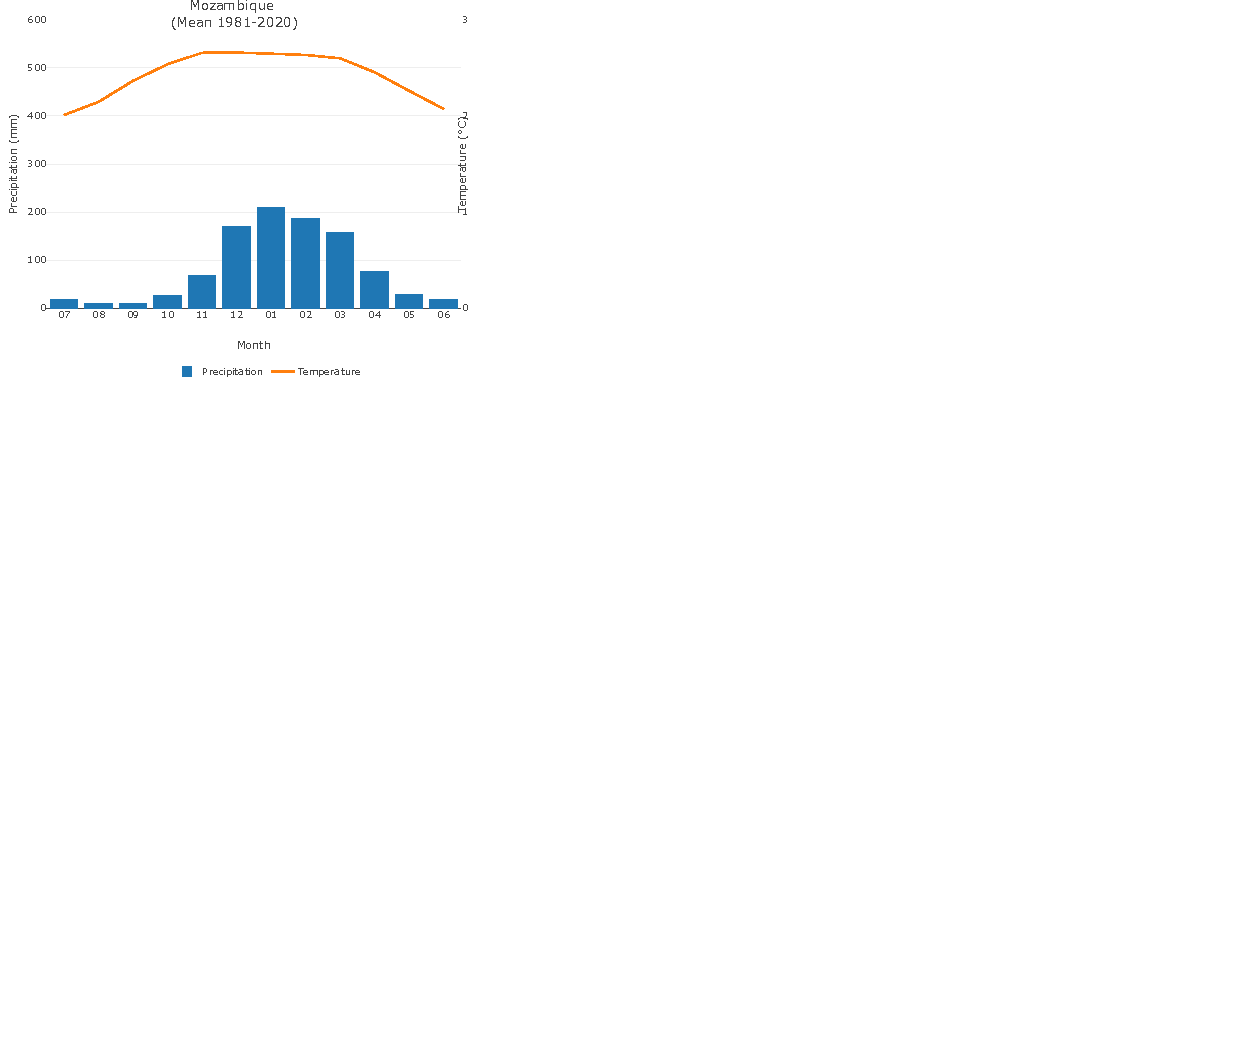
\includegraphics{Mozambique-NAP_files/figure-latex/unnamed-chunk-4-1.pdf}

\hypertarget{cabo-delgado}{%
\subsection{Cabo Delgado}\label{cabo-delgado}}

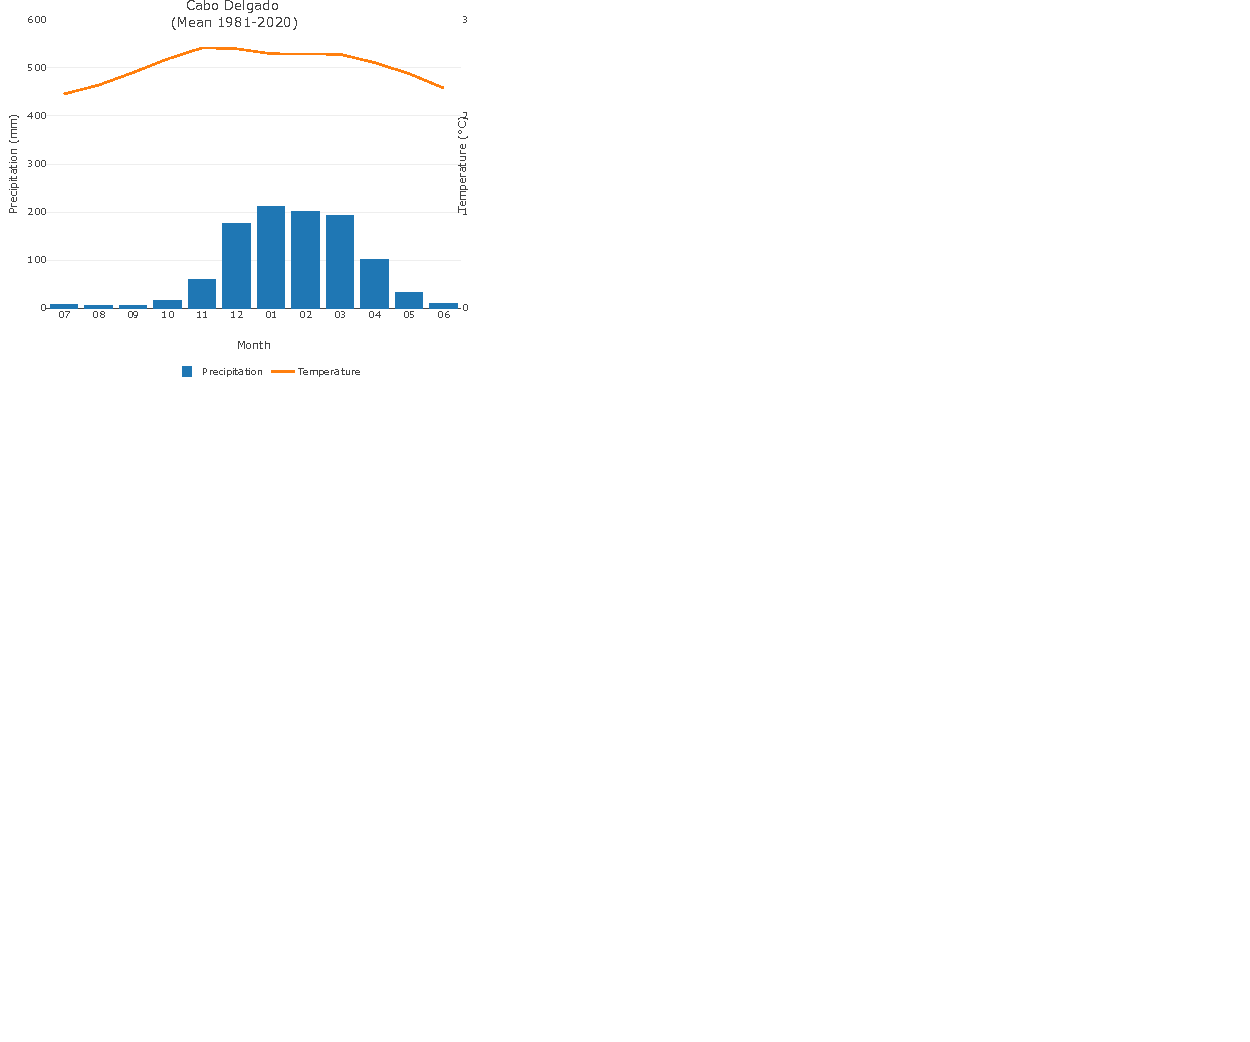
\includegraphics{Mozambique-NAP_files/figure-latex/unnamed-chunk-5-1.pdf}

\hypertarget{sofala}{%
\subsection{Sofala}\label{sofala}}

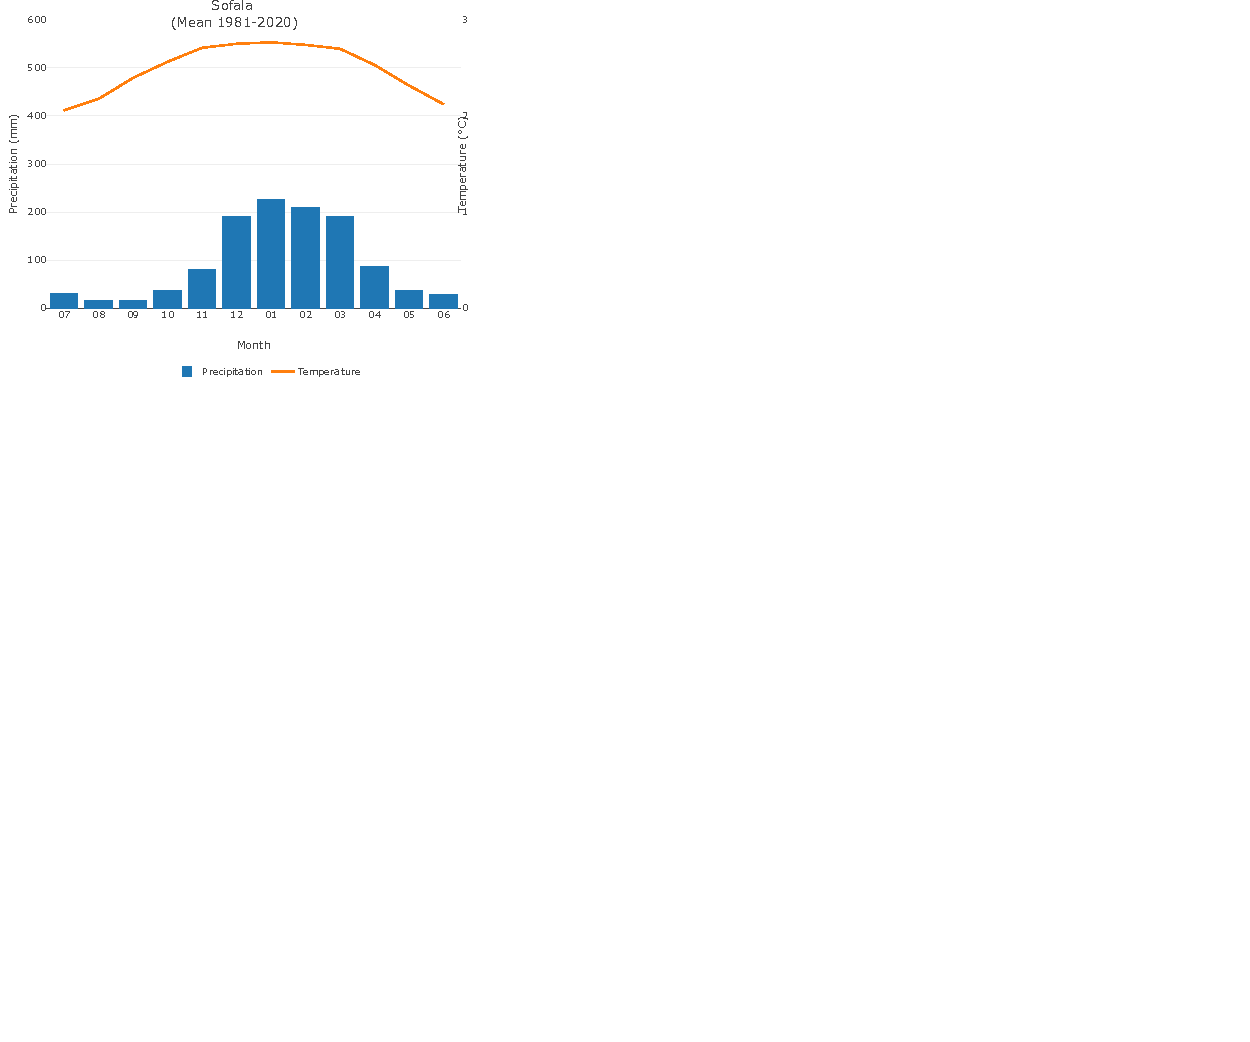
\includegraphics{Mozambique-NAP_files/figure-latex/unnamed-chunk-6-1.pdf}

\hypertarget{gaza}{%
\subsection{Gaza}\label{gaza}}

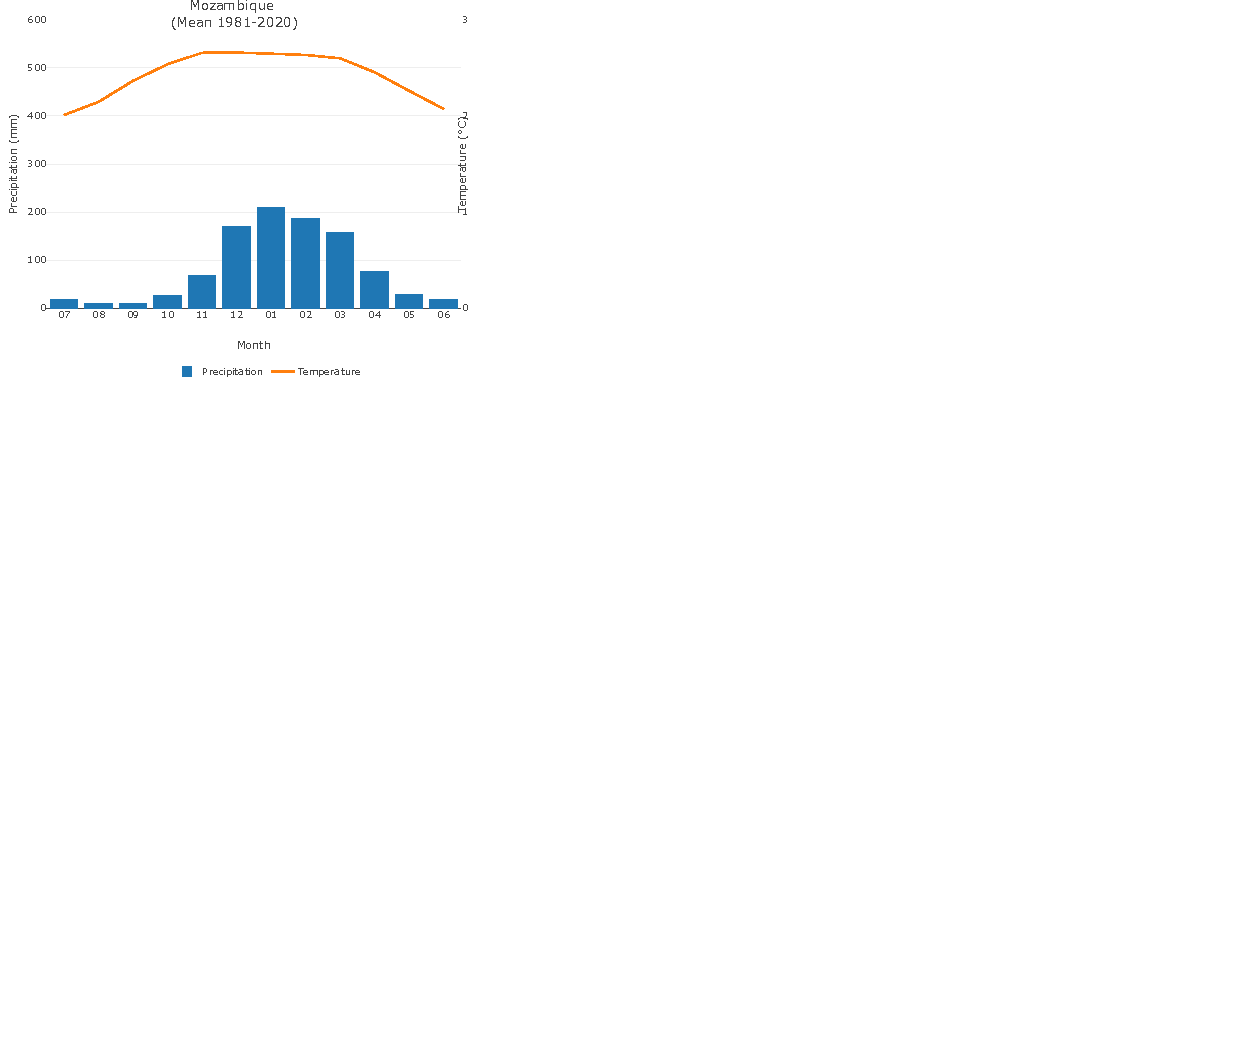
\includegraphics{Mozambique-NAP_files/figure-latex/unnamed-chunk-7-1.pdf}

\hypertarget{inhambane}{%
\subsection{Inhambane}\label{inhambane}}

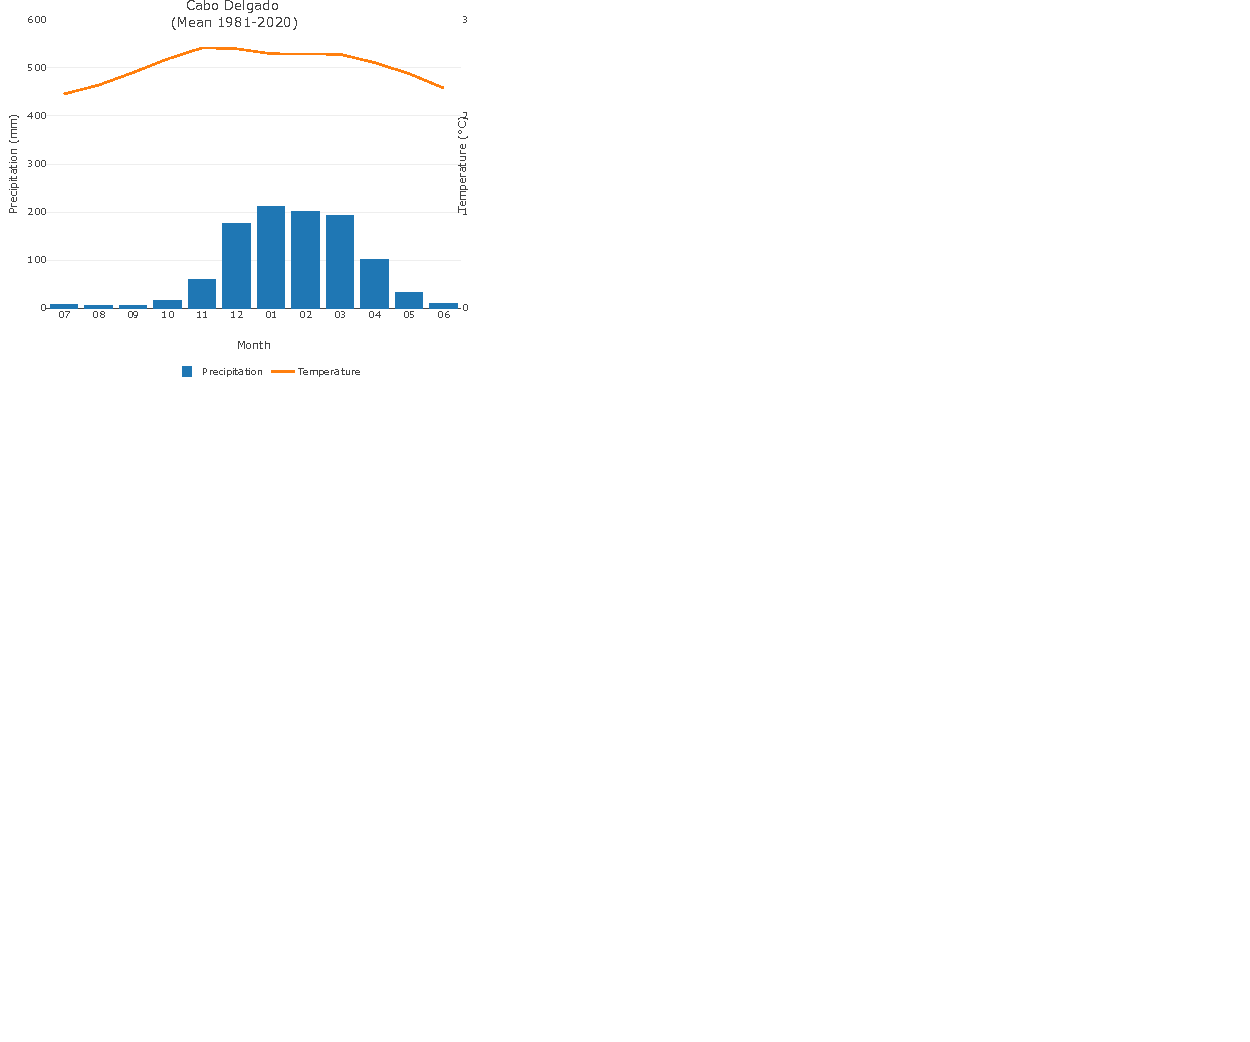
\includegraphics{Mozambique-NAP_files/figure-latex/unnamed-chunk-8-1.pdf}

\hypertarget{manica}{%
\subsection{Manica}\label{manica}}

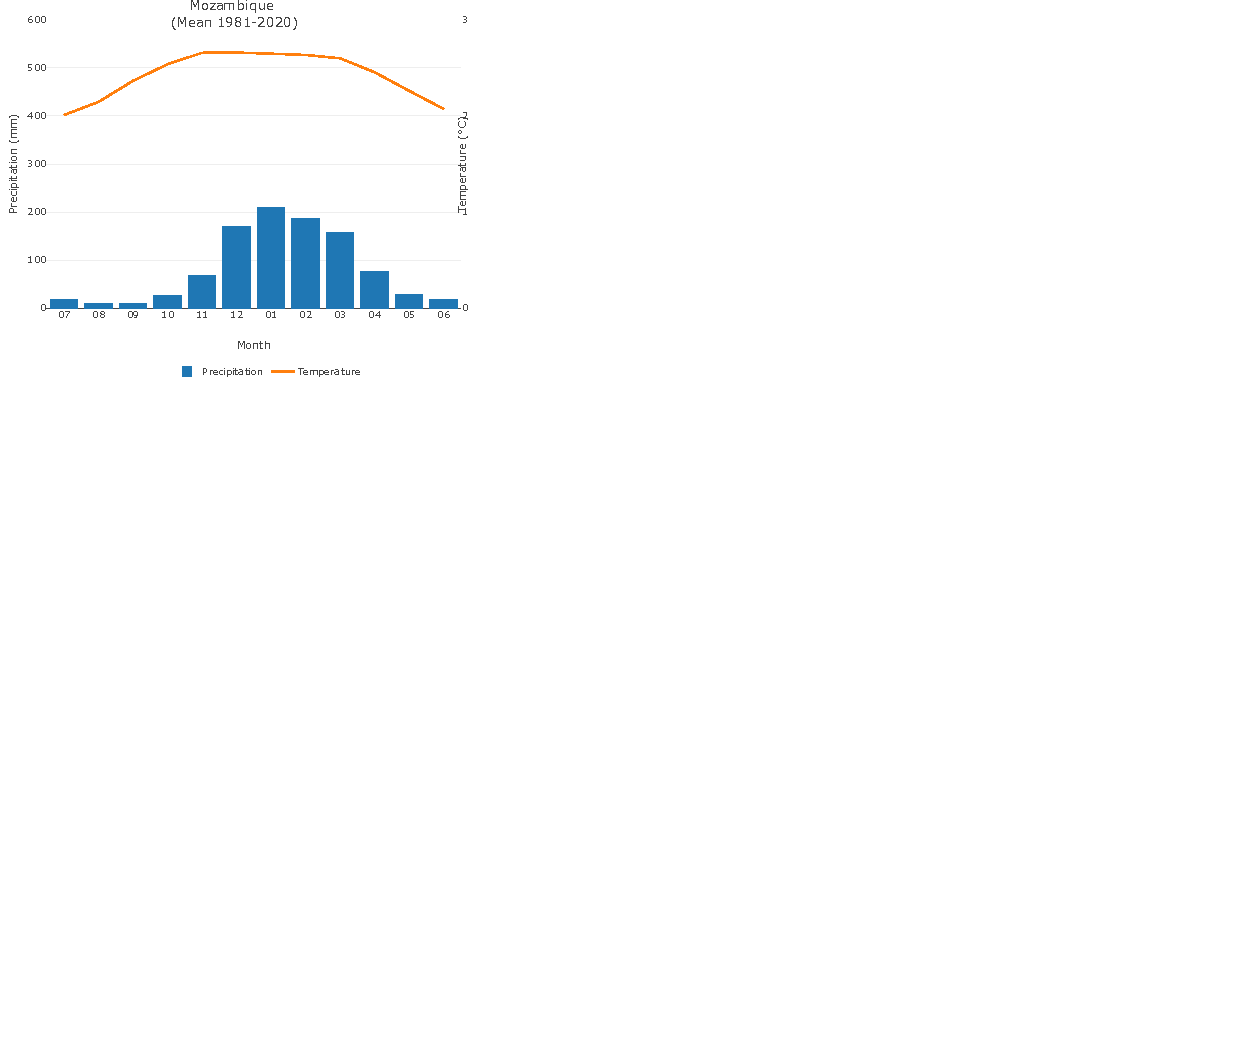
\includegraphics{Mozambique-NAP_files/figure-latex/unnamed-chunk-9-1.pdf}

\hypertarget{maputo}{%
\subsection{Maputo}\label{maputo}}

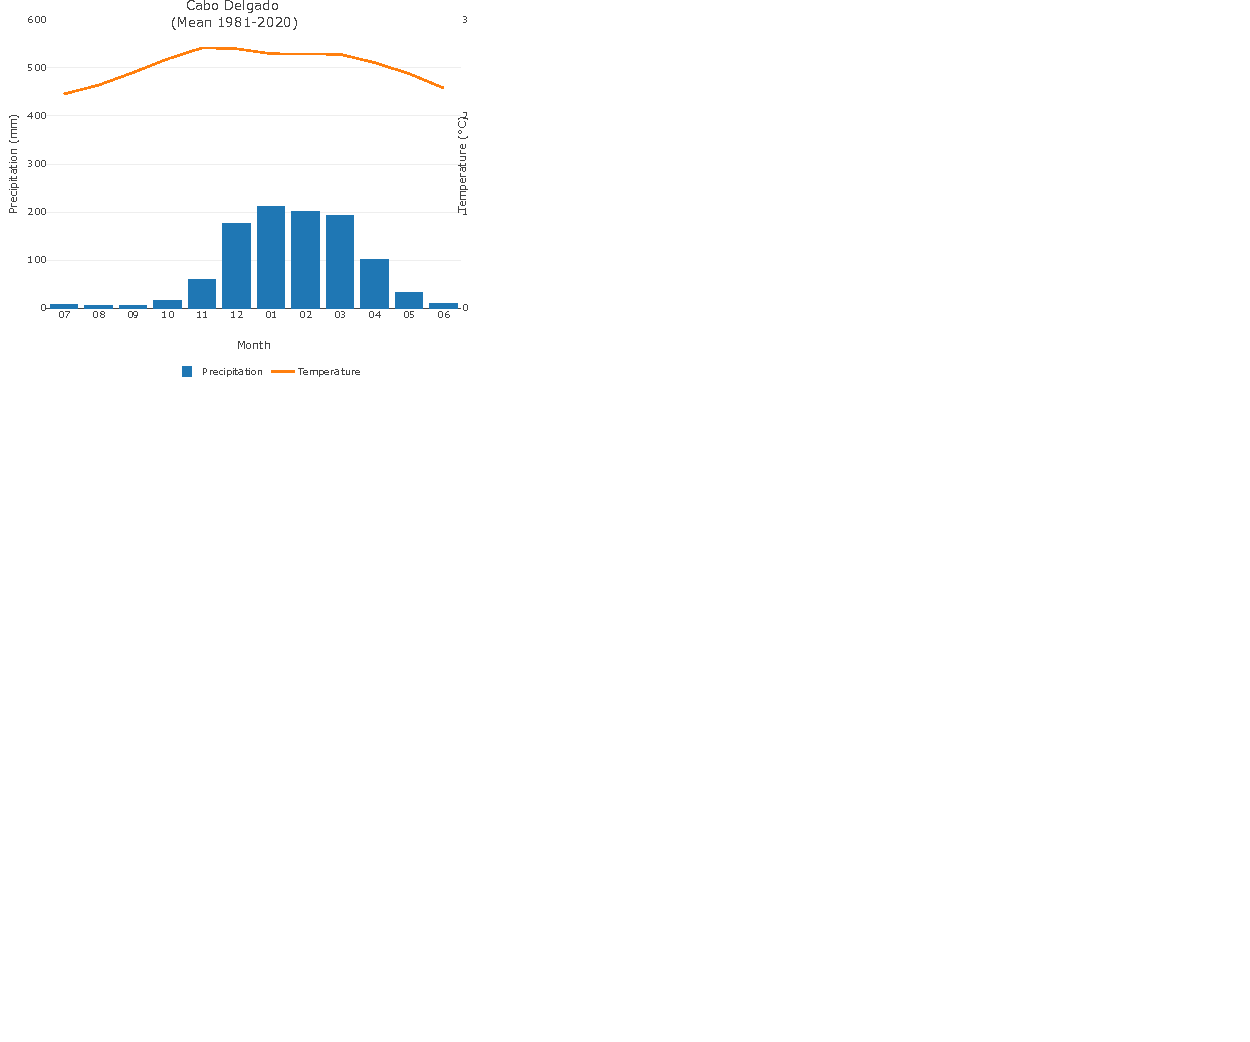
\includegraphics{Mozambique-NAP_files/figure-latex/unnamed-chunk-10-1.pdf}

\hypertarget{section}{%
\subsection{}\label{section}}

\hypertarget{nampula}{%
\subsection{Nampula}\label{nampula}}

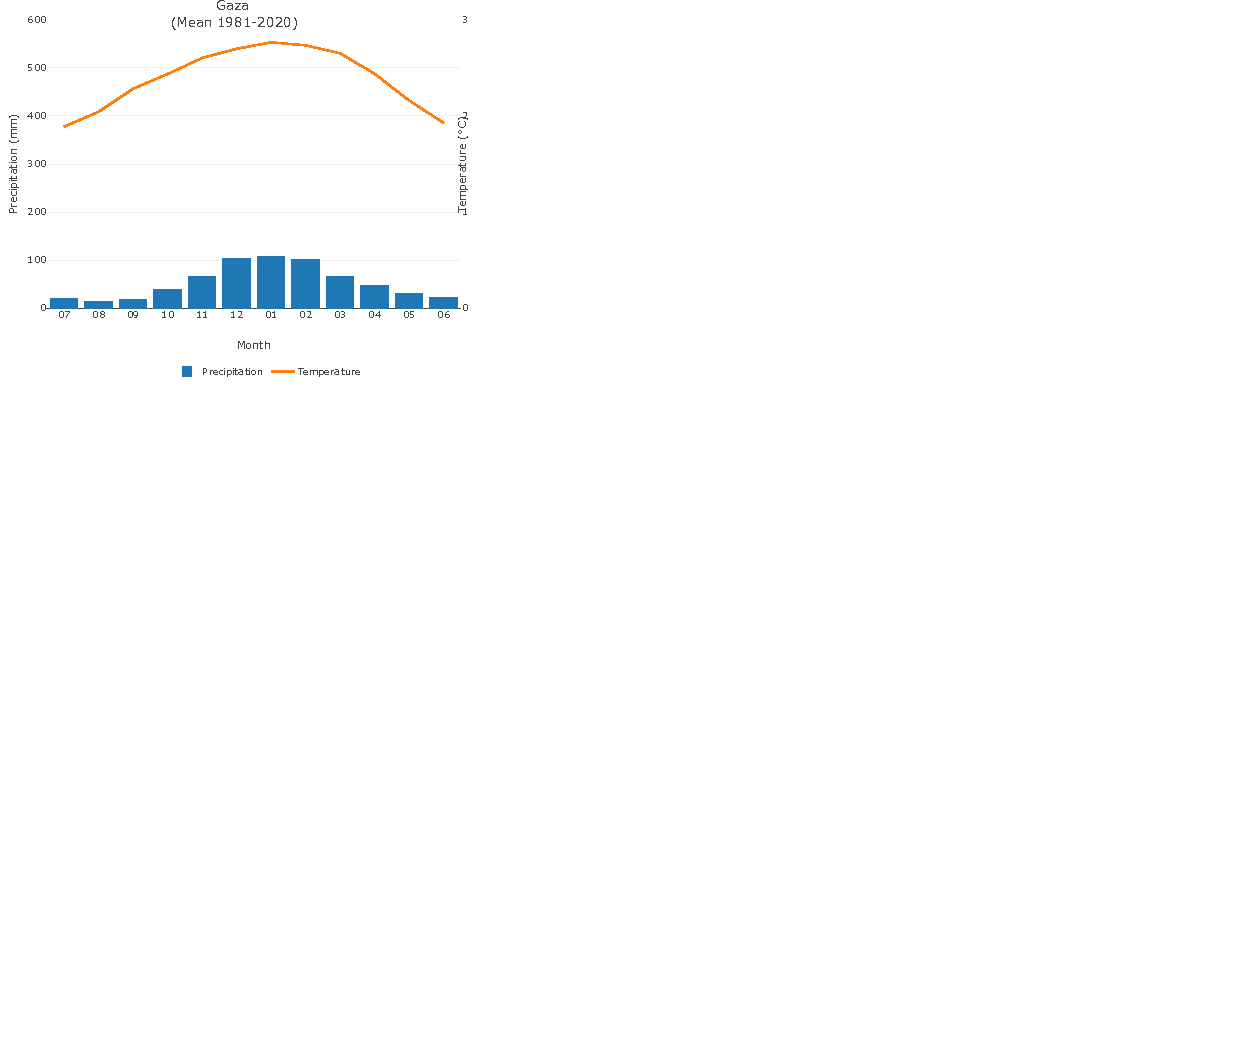
\includegraphics{Mozambique-NAP_files/figure-latex/unnamed-chunk-12-1.pdf}

\hypertarget{nassa}{%
\subsection{Nassa}\label{nassa}}

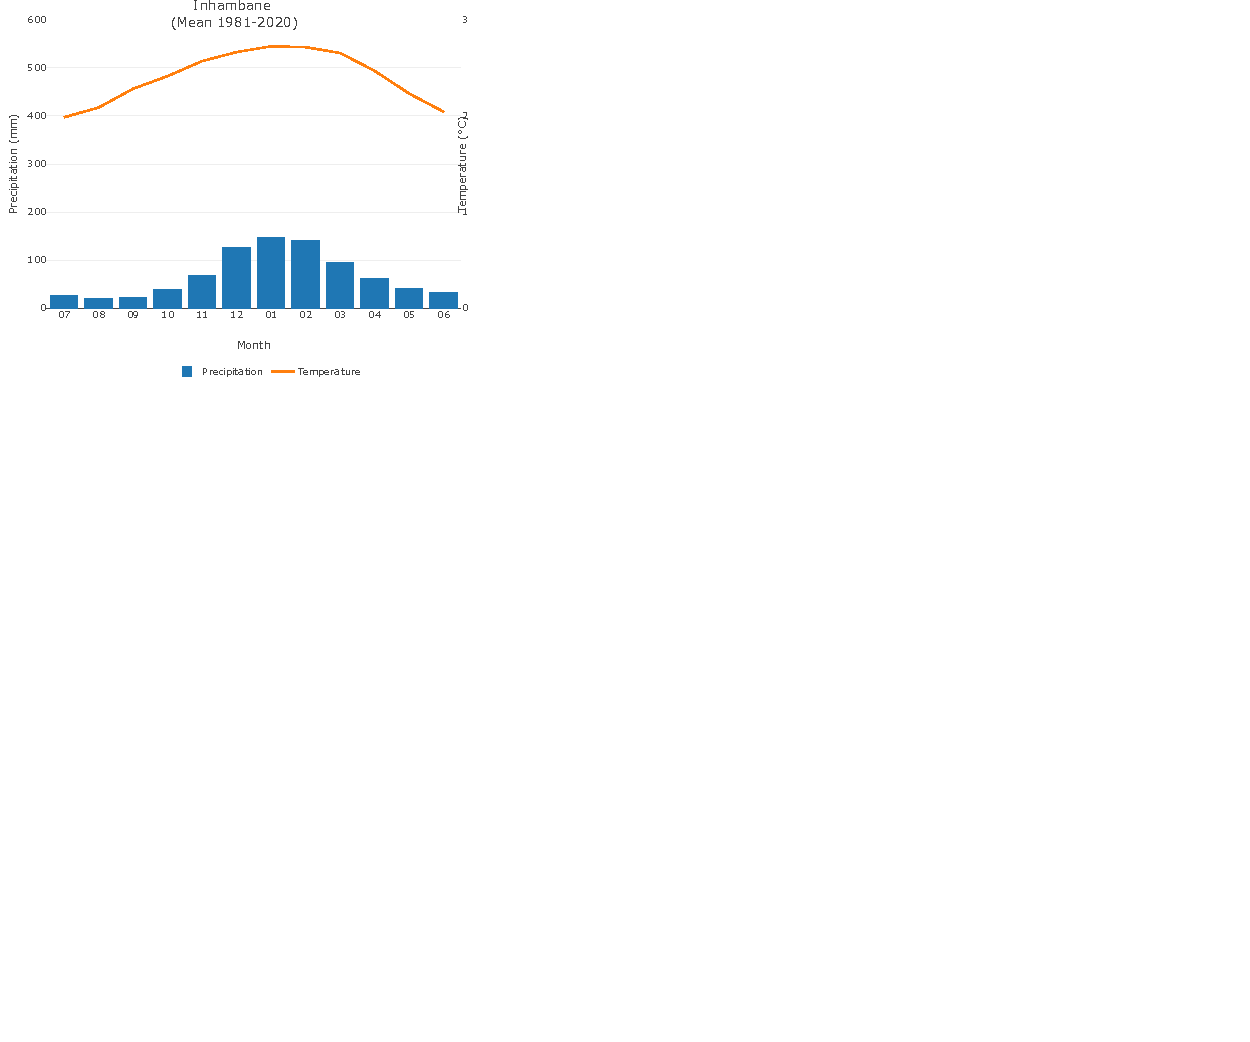
\includegraphics{Mozambique-NAP_files/figure-latex/unnamed-chunk-13-1.pdf}

\hypertarget{tete}{%
\subsection{Tete}\label{tete}}

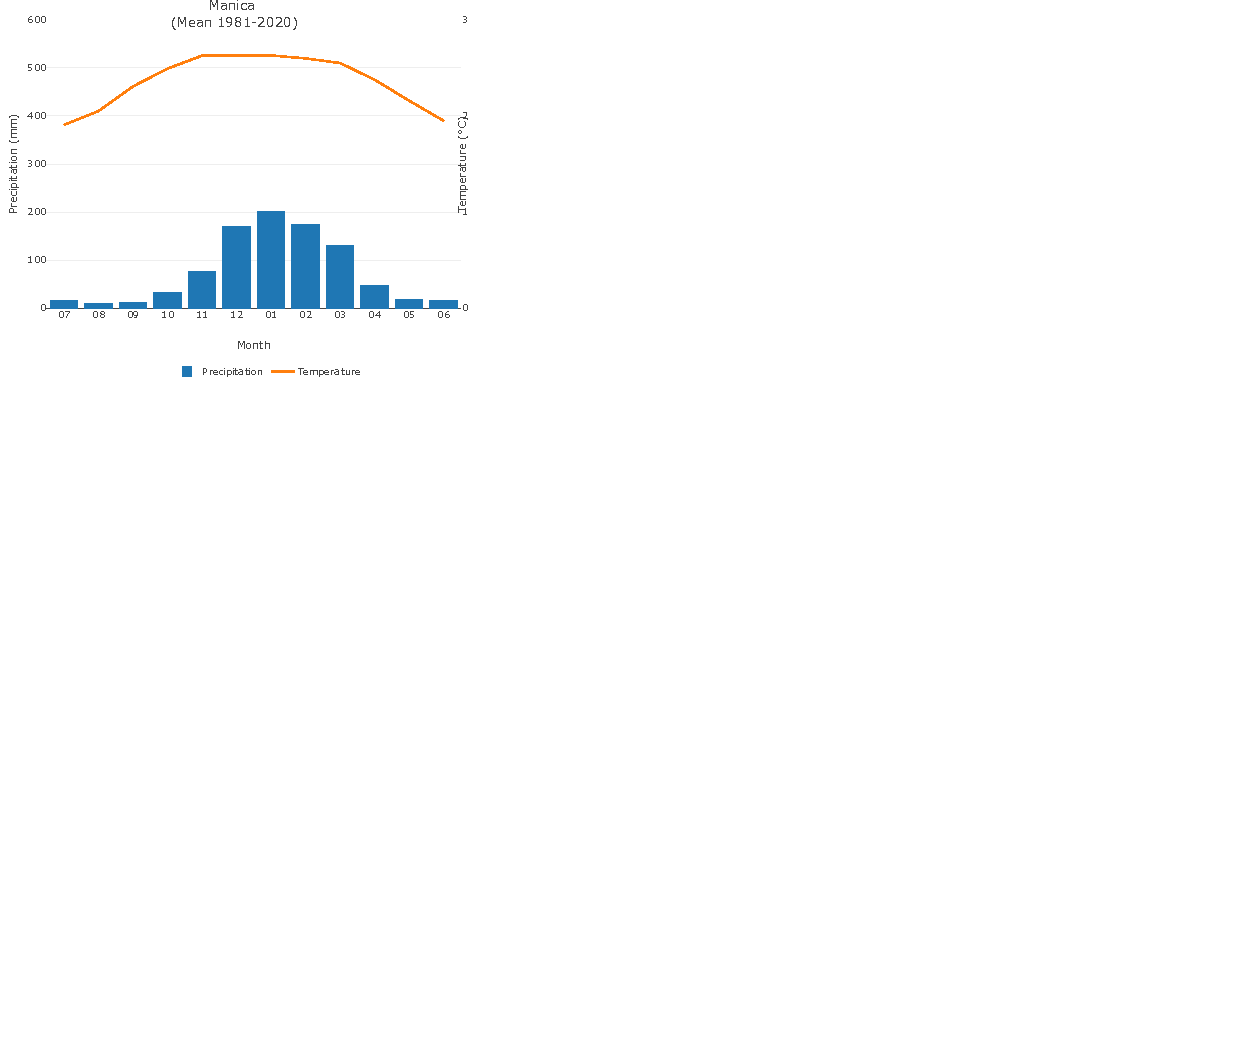
\includegraphics{Mozambique-NAP_files/figure-latex/unnamed-chunk-14-1.pdf}

\hypertarget{zambezia}{%
\subsection{Zambezia}\label{zambezia}}

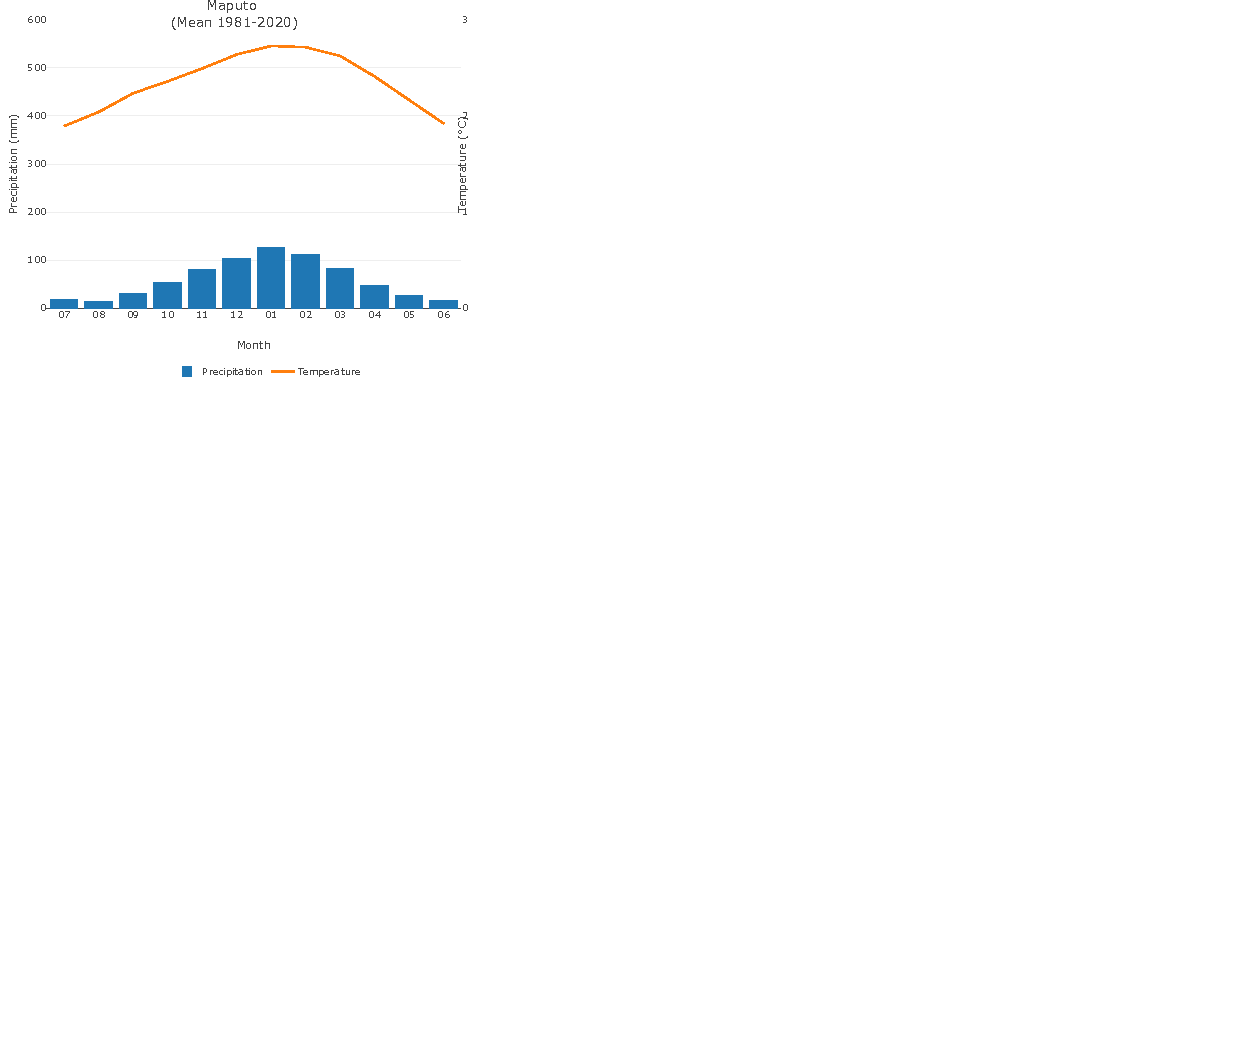
\includegraphics{Mozambique-NAP_files/figure-latex/unnamed-chunk-15-1.pdf}

\hypertarget{temperature-anomaly}{%
\section{Temperature Anomaly}\label{temperature-anomaly}}

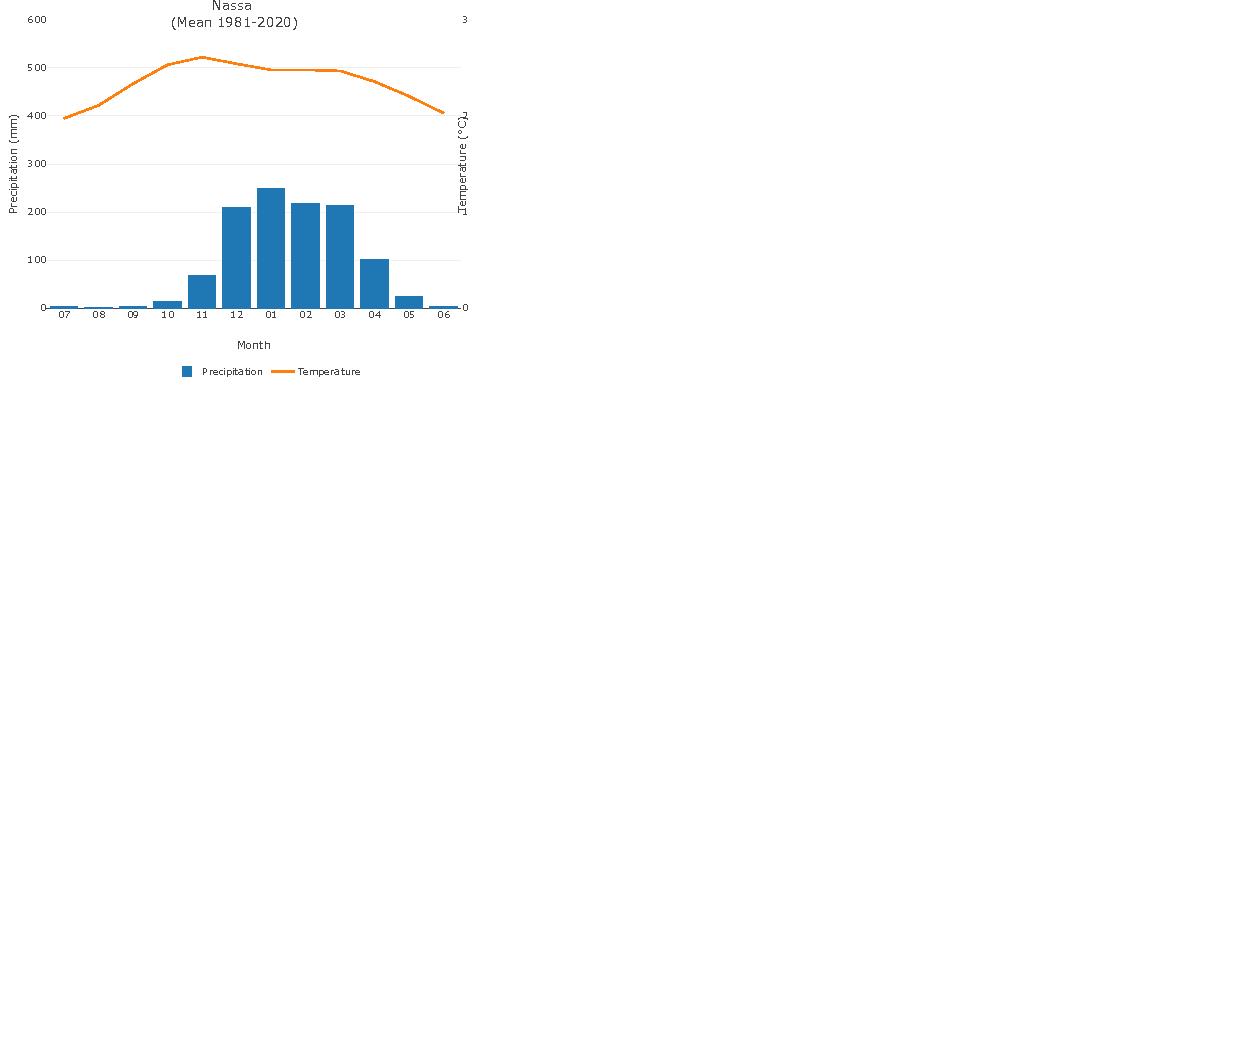
\includegraphics{Mozambique-NAP_files/figure-latex/unnamed-chunk-16-1.pdf}

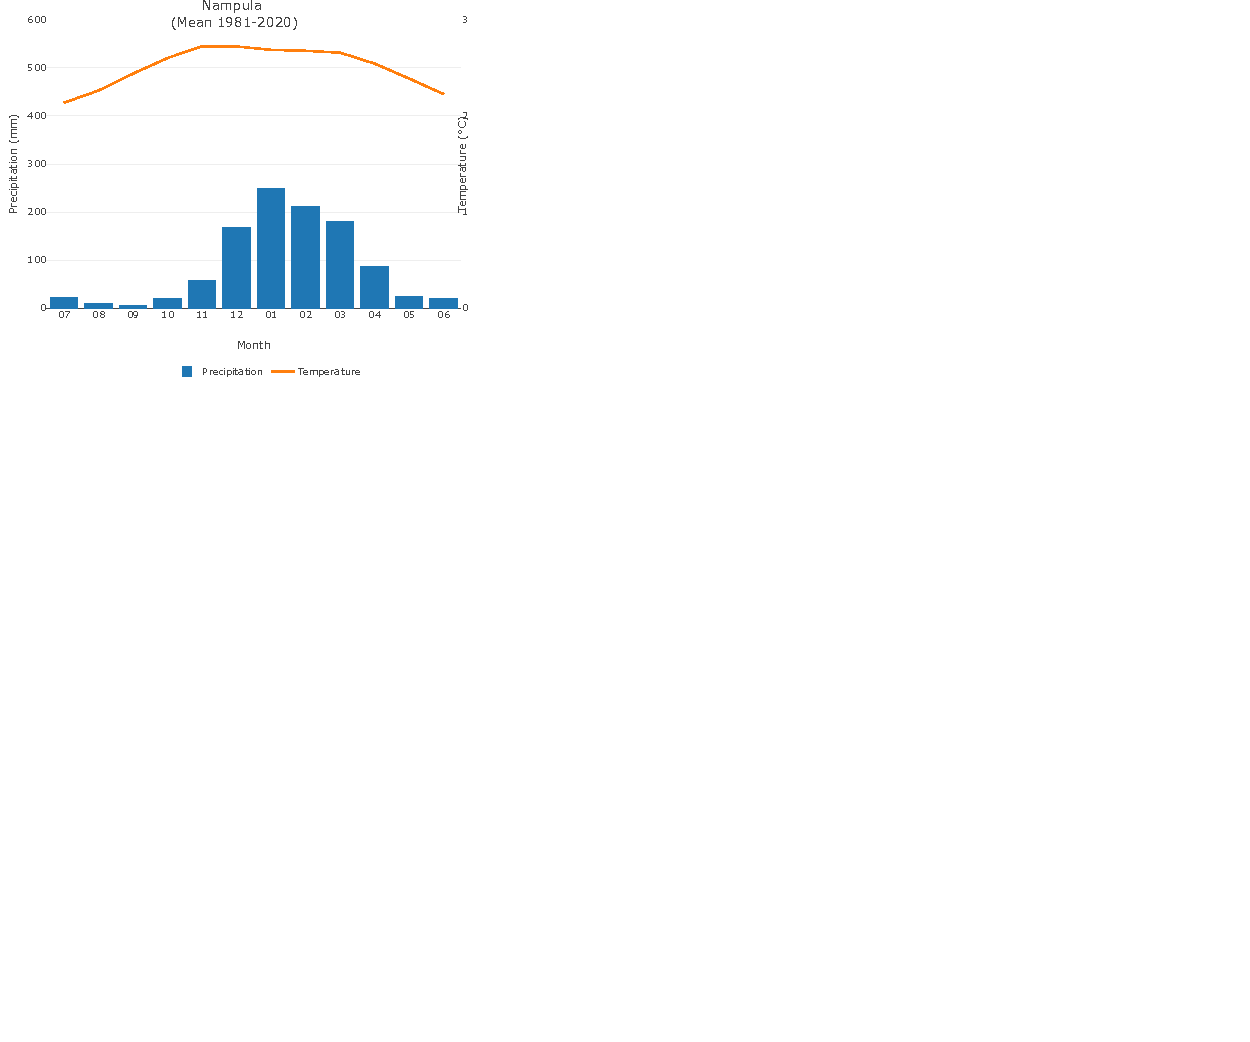
\includegraphics{Mozambique-NAP_files/figure-latex/unnamed-chunk-17-1.pdf}

\hypertarget{current-impacts-vulnerabilities-and-risks}{%
\section{Current impacts, vulnerabilities and risks}\label{current-impacts-vulnerabilities-and-risks}}

Dados históricos sobre eventos extremos mostram que três riscos relacionados com o clima são mais prováveis de ocorrer em Moçambique, a saber, ciclones tropicais, inundações e secas. Estes eventos são frequentemente associados a danos socioeconómicos, traduzidos em perdas de vidas humanas, sofrimento humano, perda de bens, destruição de infraestruturas críticas (ex. unidades sanitárias, escolas, vias de acesso, etc.) e outras perdas indirectas.
Uma análise de dados no período de 1980 a 2019 mostra que Moçambique foi afectado por 21 ciclones tropicais, 20 eventos de inundação e 12 secas (figura 3.1). Isto significa que em média, o país é afectado por um ciclone tropical ou um evento de inundação a cada dois anos e um evento de seca a cada três anos. Os ciclones tropicais e os eventos de inundações representam cerca de 77\% do total dos eventos ocorridos no período em análise.

\begin{figure}
\centering
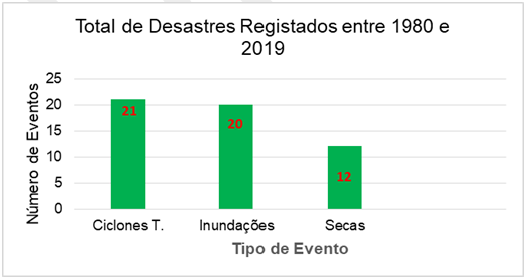
\includegraphics{images/numero_desastres.png}
\caption{Figura 3.1:-Número total de eventos extremos ocorridos em Moçambique, entre 1980 -- 2019}
\end{figure}

(Fonte: produzido com base nos dados do DeSinventar e relatórios do INGC de balanço da época chuvosa).

Uma das questões cruciais da actualidade é se existe alguma evidência do aumento ou não dos eventos extremos causadores de desastres. Através de uma análise da tendência dos eventos registados nas últimas quatro décadas (1980 -- 2019), nota-se que o número de eventos que assolaram o país aumentou, significativamente, desde a década 2000 (figura 3.2). Desde a década de (2000-2010) até à corrente, o número de ciclones concorre com o número de eventos de inundação, apesar do abrandamento dos eventos de seca.
Tomando em conta que os ciclones tropicais são frequentemente associados a eventos de chuvas fortes que podem contribuir com uma proporção significativa da precipitação em um período muito curto que por sua vez causam inundações em várias regiões do país, com sérias implicações para a saúde das comunidades, o agravamento destes fenómenos nas últimas décadas deve merecer uma atenção especial para as autoridades da saúde e não só.

\begin{figure}
\centering
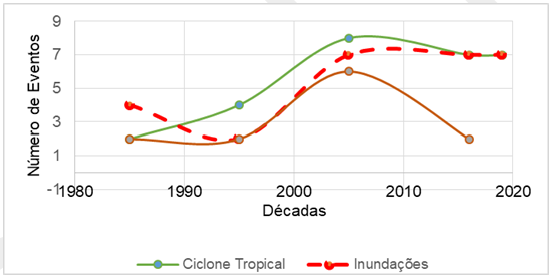
\includegraphics{images/eventos_extremos.png}
\caption{Figura 3.2: Tendência do número de eventos extremos ocorridos entre 1980 e 2019.}
\end{figure}

O impacto directo destes eventos é frequentemente expresso pelo número da perda de vidas humanas, pessoas afectadas através da perda de bens pessoais e meios de subsistência, destruição de infra-estruturas críticas do país tais como estradas, pontes, sistema de abastecimento de água, escolas, hospitais, assim como a eclosão de doenças transmitidas pela água (ex. malária, cólera, diarreias etc.). Todavia, a falta de registos sistemáticos e homogéneos dos eventos e seus impactos e, por um lado, a persistência em se considerar apenas os desastres de grandes proporções e elevado impacto num curto espaço de tempo, têm ocultado milhares de desastres de pequena e média escala que ocorrem todos os anos no país. Consequentemente, Moçambique não conhece o valor real das perdas económicas directas e ou indirectas associadas a estes eventos.

A Tabela 3.1 apresenta o impacto das mudanças climáticas na dimensão humana. Relativamente aos impactos económicos, estes são apresentados nos respectivos sectores onde é feita a análise da vulnerabilidade.

\#\#\#\#\#\#\#\#\#\#\#\#\#\#\#table\#\#\#\#\#\#\#\#\#\#\#\#\#\#\#

Os eventos climáticos extremos ocorridos em Moçambique em 2000 e nas épocas chuvosas de 2005/6 a 2017/18 afectaram cerca de 4,074,606 pessoas, causaram ferimentos a 885 pessoas e 1,114 óbitos. Cerca de 50\% de afectados, feridos e óbitos resultaram da ocorrência do Ciclone HUDAH, e importa referir que os ciclones tropicais são eventos que provocam maiores impactos na dimensão humana.
Estes impactos constituem um retrocesso no processo de redução da pobreza que é a prioridade dos Governos dos países em vias de desenvolvimento e aumentam a dependência pela ajuda internacional. Neste contexto, é de alta prioridade a avaliação da vulnerabilidade dos sectores sociais e económicos mais importantes e a identificação de medidas de adaptação.

\textbf{Agricultura}

De acordo com os balanços das épocas chuvosas, o sector de agricultura é vulnerável aos eventos de estiagem e secas, cheias e inundações, ventos fortes, ciclones tropicais incluindo pragas (vide a Tabela 3.3). Estes eventos resultam em áreas de culturas afectadas e/ou perdidas; morte e/ou desaparecimento de animais domésticos, com destaque para o gado bovino, caprino, suíno, ovino e aves; destruição de infra-estruturas agrárias e de maneio dos animais; perda de áreas de pastagem, afectando os agricultores e suas famílias.
Tabela 3.3: Impacto das mudanças climáticas na agricultura

\#\#\#\#\#\#\#\#\#\#\#\#\#\#\#\#\#\#\#\#3table\#\#\#\#\#\#\#\#\#\#\#\#\#3

\emph{Fonte: Balanços das épocas chuvosas do período de 2011-12 a 2017-18}

Os eventos climáticos ocorridos no país entre as épocas chuvosas de 2011-12 a 2017-18 afectaram cerca de 1,384,677 ha de culturas, dos quais cerca de 733,270 ha foram perdidas. Os eventos que afectaram maior área de culturas foram a depressão tropical Dando e o ciclone tropical Funso, ocorridos na época chuvosa 2011-12, enquanto a maior perda de culturas ocorreu na sequência das inundações de 2012-2013.
Para além de áreas afectadas e/ou perdidas de culturas, os eventos climáticos ocorridos no país causaram morte de 315 cabeças de gado bovino, 2,707 de caprinos, 254 suínos, 111 ovinos e 132 aves. Em termos de equipamentos, 9 represas e 113 motobombas foram danificados. Estas perdas e destruições afectaram 278,394 produtores e cerca de 25 mil famílias.\\
Os eventos que mais perdas e destruições causam no sector de agricultura são os relacionados com excessos de chuvas e inundações e os ciclones tropicais. Contudo, quando ocorre uma estiagem, normalmente, a área afectada é igual a perdida.\\
É importante sublinhar também que além da vulnerabilidade biofísica associada à ocorrência de eventos climáticos extremos, os níveis de tecnologia adoptados por grande parte dos produtores não correspondem às exigências das variedades seleccionadas, devido à fraca capacidade financeira para aquisição de insumos agrícolas, o que também contribui para a baixa produção e produtividade.\\
Para a avaliação da vulnerabilidade do sector agrícola às mudanças climáticas foi seleccionada a cultura de milho produzida em sequeiro, no distrito de Chókwé, província de Gaza. A avaliação consistiu na análise da relação entre o rendimento da cultura e as variáveis climáticas (precipitação e temperatura) e feita a projecção das variáveis climáticas e seus possíveis impactos nos rendimentos.

Pecuária

Tabela 3.4: Impactos dos eventos extremos na pecuária

\#\#\#\#\#\#\#\#\#\#\#\#\#\#3table\#\#\#\#\#\#\#\#\#\#\#\#\#

\hypertarget{projected-future-impacts-vulnerabilities-and-risks}{%
\section{Projected future impacts, vulnerabilities and risks}\label{projected-future-impacts-vulnerabilities-and-risks}}

Em Moçambique, alguns estudos apontam para um aumento significativo para a temperatura, sendo que a temperatura média anual está projectada para aumentar entre 1.0 a 2.8 °C por volta de 2060 e entre 1.4 a 4.6 ° C em 2090 (INGC, 2009; Mcsweeney et al., 2010) (igura 1.10). A taxa projectada de aquecimento será mais rápida nas regiões interiores de Moçambique do que nas áreas mais próximas da costa. Todas as projecções indicam aumentos substanciais na frequência de dias e noites considerados ``quentes'' no clima actual. Sendo que este aumento estará entre 17 e 35\% de dias por ano, por volta de 2060 e entre 20 e 53\% de dias por ano em 2090. As mesmas projecções indicam também uma redução na frequência de dias e noites consideradas ``frias'' no clima actual.

\hypertarget{temperature}{%
\subsection{Temperature}\label{temperature}}

\begin{figure}
\centering
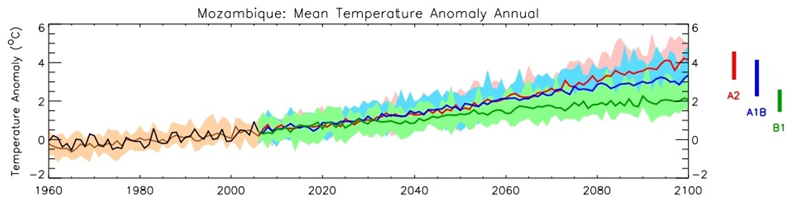
\includegraphics{images/temp_anomaly.png}
\caption{Figura 1.10: Tendências da temperatura média anual em Moçambique para o passado recente entre 1960 e 2006 (linha em preto) e o futuro projectado para três cenários de emissões (linhas coloridas). As barras coloridas no lado direito indicam os diferentes cenários usados nas simulações (A2, A1B e B1) assim como as faixas de incertezas nas projecções de climas médios por volta de 2090 -- 2100 (Adaptado de Mcsweeney et al., 2010).}
\end{figure}

\hypertarget{ssp245}{%
\subsubsection{ssp245}\label{ssp245}}

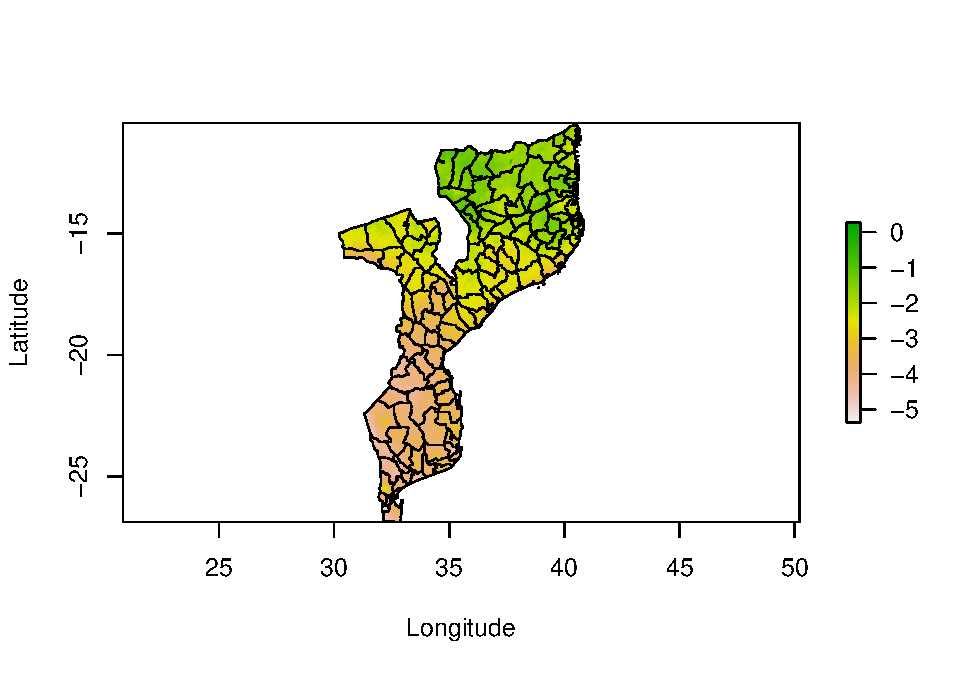
\includegraphics{Mozambique-NAP_files/figure-latex/ssp245-national-1.pdf}

Fig. 4a. Mean temperature change (C) for Mozambique for 2020 -- 2040 compared to reference period 1971 -- 2000 for the medium emissions scenario (ssp245). BCC-CSM2-MR Model

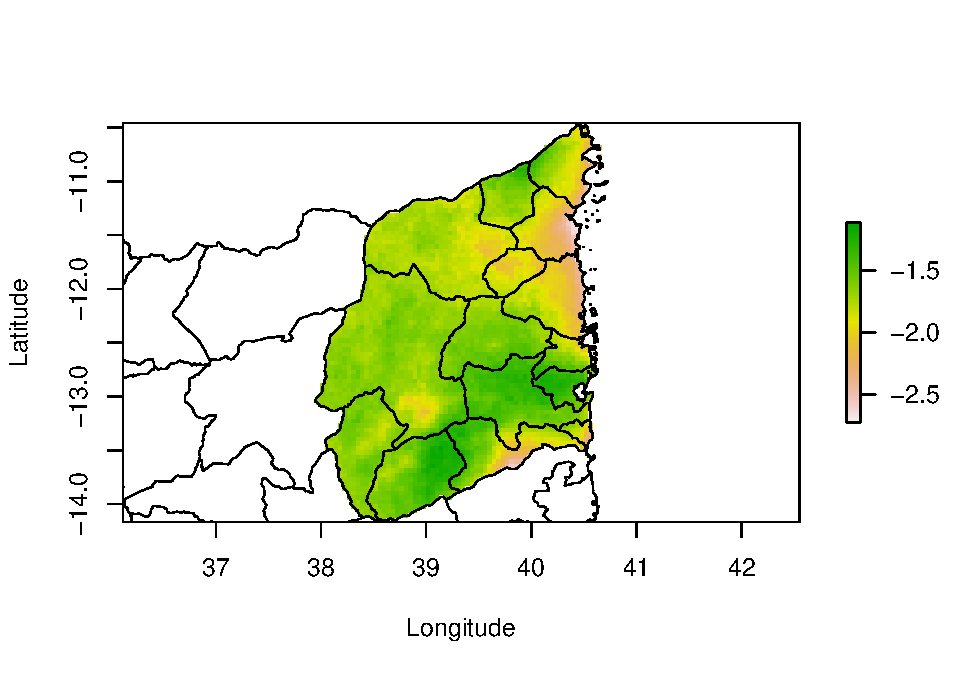
\includegraphics{Mozambique-NAP_files/figure-latex/ssp245-cabo-1.pdf}

Fig. xx Mean temperature change (C) for Cabo Delgado for 2021 -- 2040 compared to reference period 1971 -- 2000 for the medium emissions scenario (ssp245). BCC-CSM2-MR Model

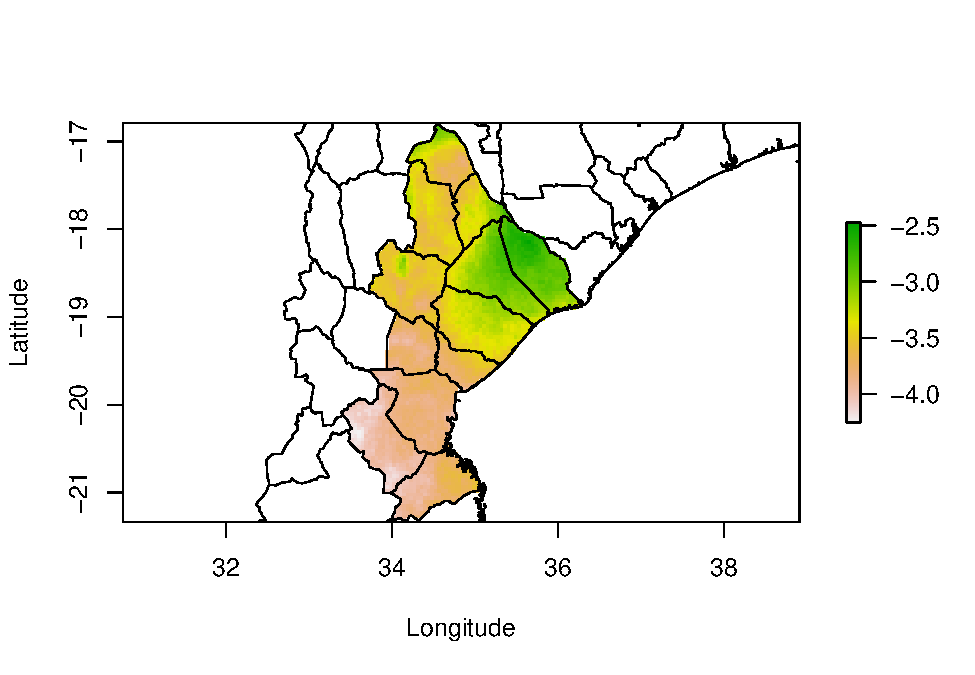
\includegraphics{Mozambique-NAP_files/figure-latex/ssp245-sofala-1.pdf}

Fig. xx Mean temperature change (C) for maputo for 2021 -- 2040 compared to reference period 1971 -- 2000 for the medium emissions scenario (ssp245). BCC-CSM2-MR Model

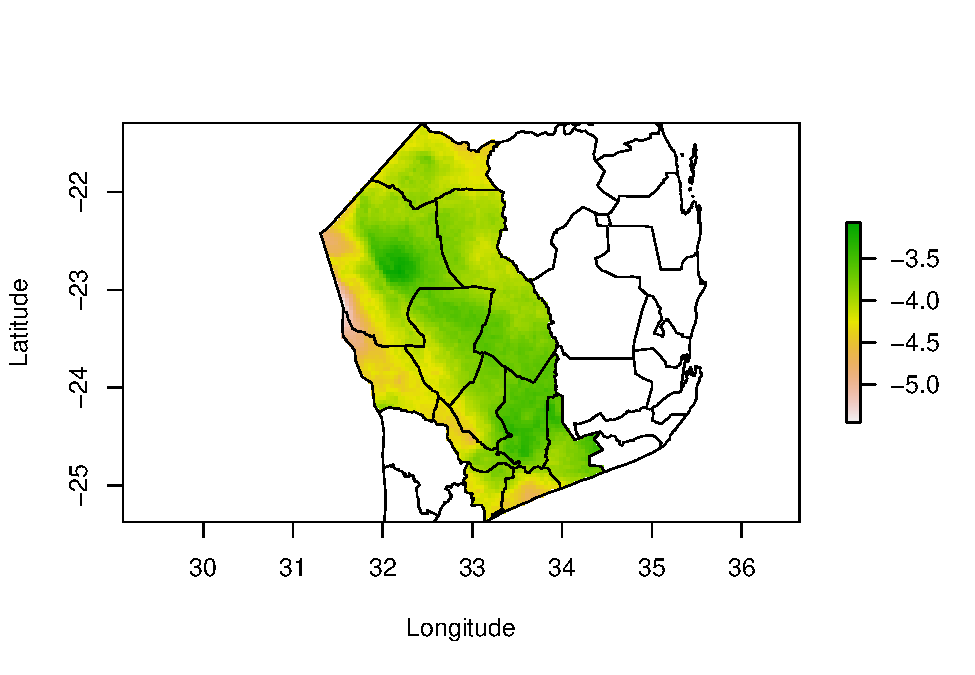
\includegraphics{Mozambique-NAP_files/figure-latex/ssp245-gaza-1.pdf}

Fig. xx Mean temperature change (C) for Gaza for 2021 -- 2040 compared to reference period 1971 -- 2000 for the medium emissions scenario (ssp245). BCC-CSM2-MR Model

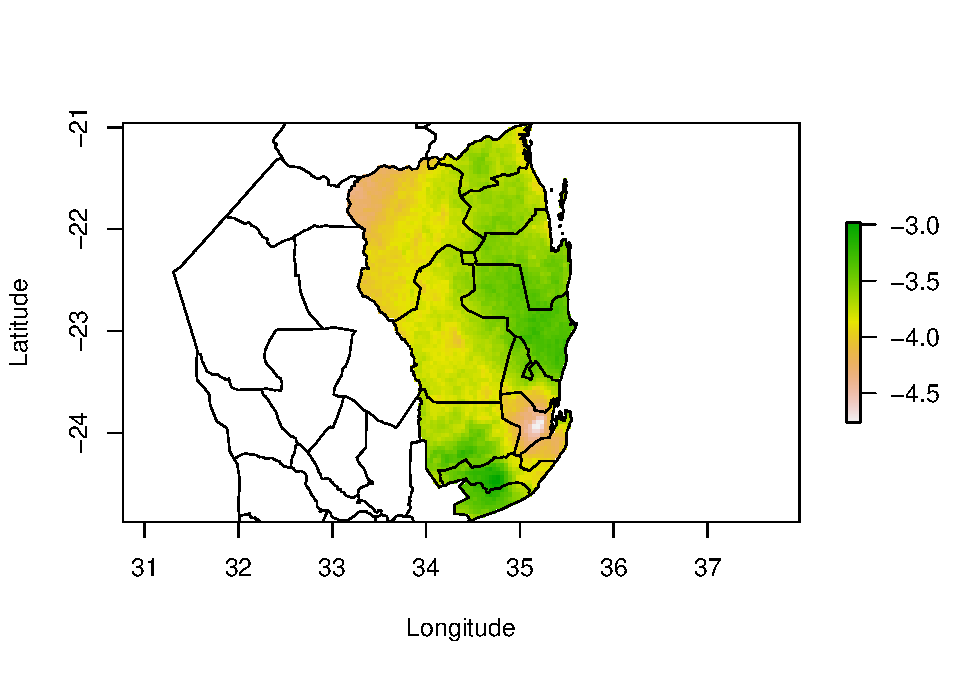
\includegraphics{Mozambique-NAP_files/figure-latex/ssp245-inbane-1.pdf}

Fig. xx Mean temperature change (C) for Inhambane for 2021 -- 2040 compared to reference period 1971 -- 2000 for the medium emissions scenario (ssp245). BCC-CSM2-MR Model

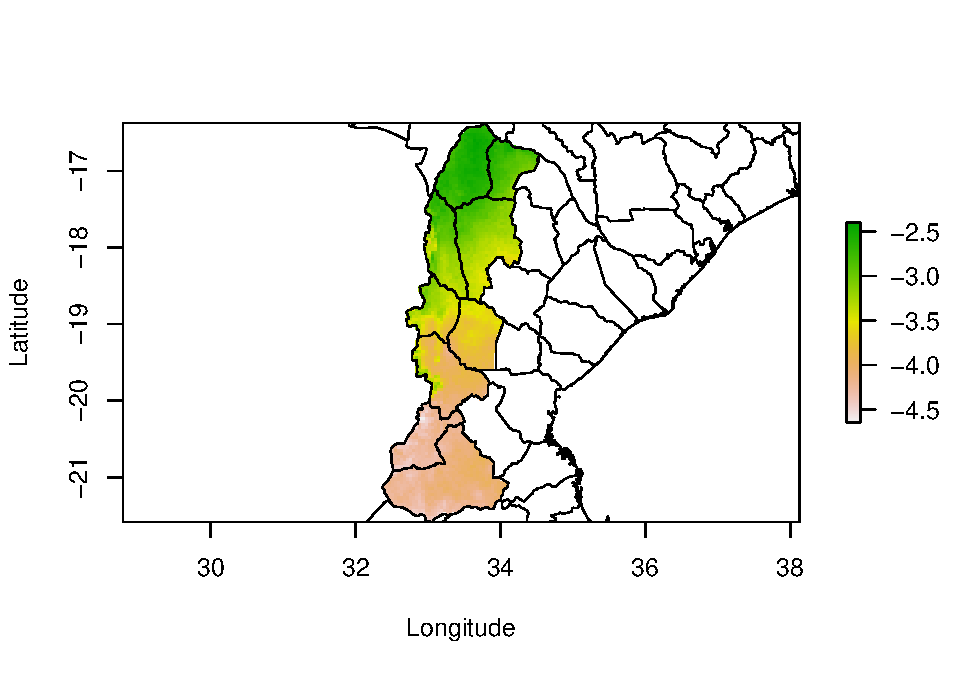
\includegraphics{Mozambique-NAP_files/figure-latex/ssp245-manica-1.pdf}

Fig. xx Mean temperature change (C) for Manica for 2021 -- 2040 compared to reference period 1971 -- 2000 for the medium emissions scenario (ssp245). BCC-CSM2-MR Model

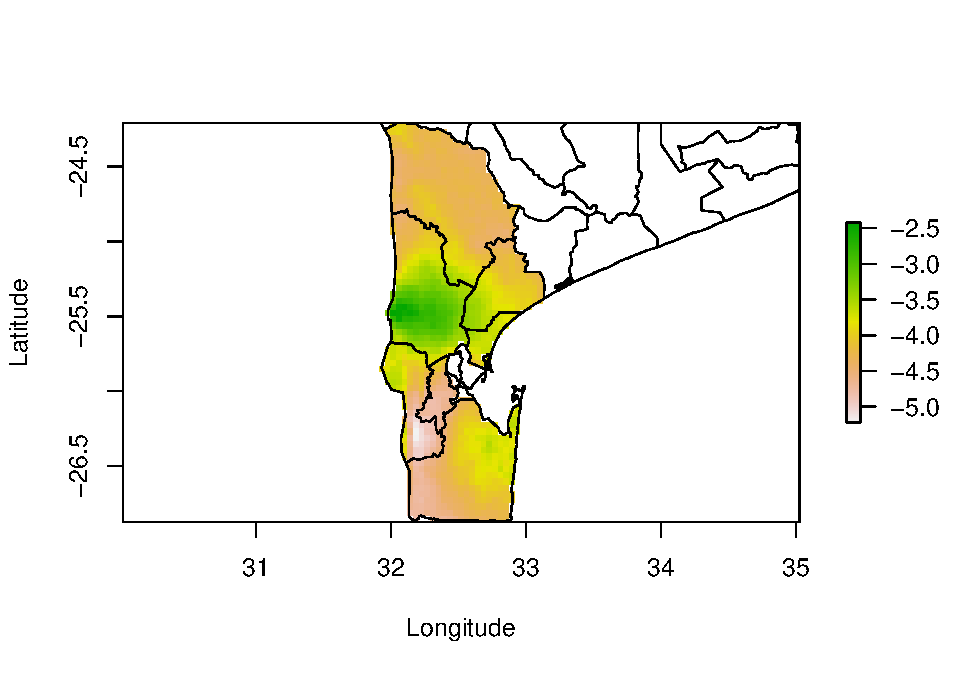
\includegraphics{Mozambique-NAP_files/figure-latex/ssp245-maputo-1.pdf}

Fig. xx Mean temperature change (C) for Maputo for 2021 -- 2040 compared to reference period 1971 -- 2000 for the medium emissions scenario (ssp245). BCC-CSM2-MR Model

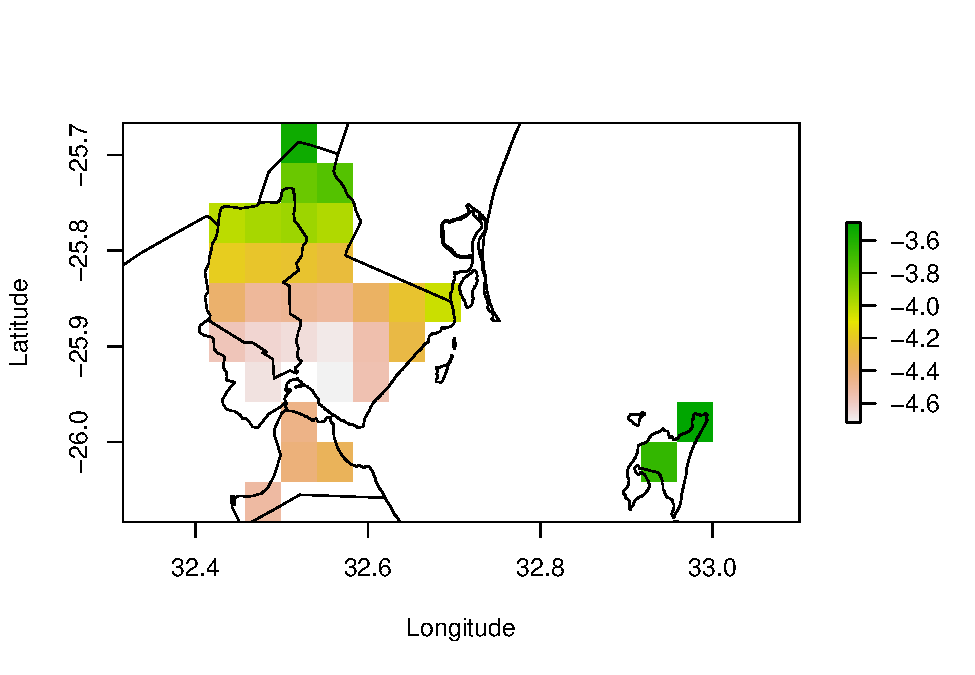
\includegraphics{Mozambique-NAP_files/figure-latex/ssp245-map.city-1.pdf}

Fig. xx Mean temperature change (C) for Maputo City for 2021 -- 2040 compared to reference period 1971 -- 2000 for the medium emissions scenario (ssp245). BCC-CSM2-MR Model

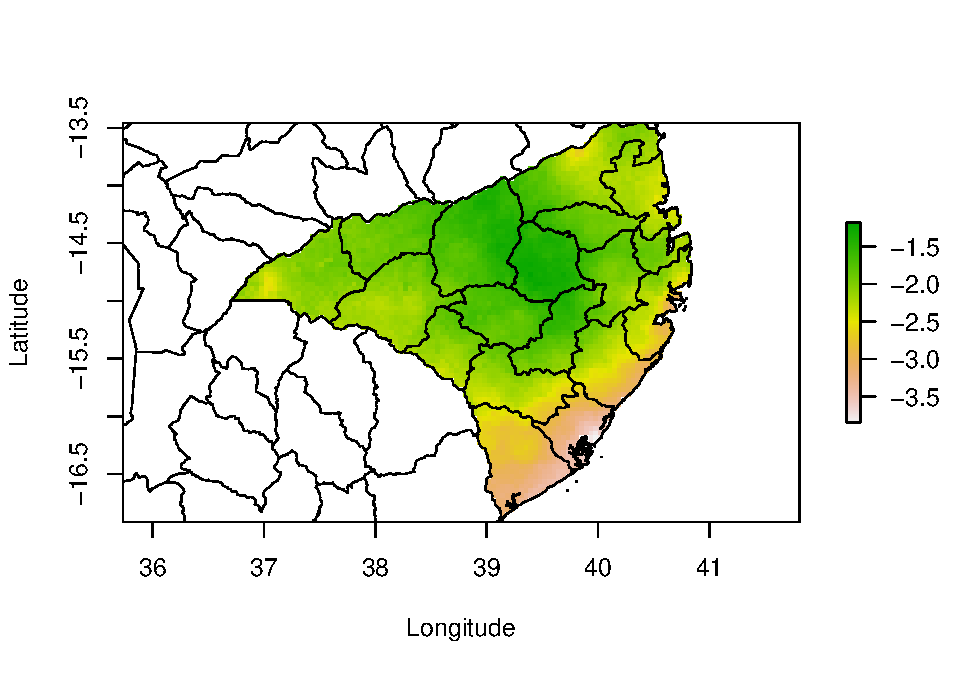
\includegraphics{Mozambique-NAP_files/figure-latex/ssp245-nampula-1.pdf}

Fig. xx Mean temperature change (C) for Nampula for 2021 -- 2040 compared to reference period 1971 -- 2000 for the medium emissions scenario (ssp245). BCC-CSM2-MR Model

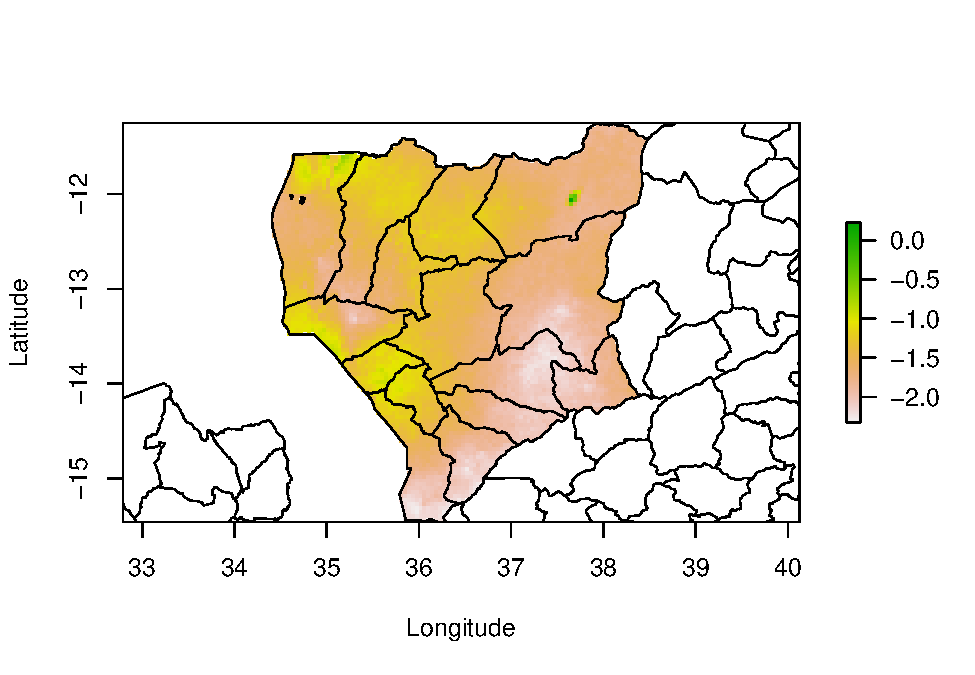
\includegraphics{Mozambique-NAP_files/figure-latex/ssp245-nassa-1.pdf}

Fig. xx Mean temperature change (C) for Nassa for 2021 -- 2040 compared to reference period 1971 -- 2000 for the medium emissions scenario (ssp245). BCC-CSM2-MR Model

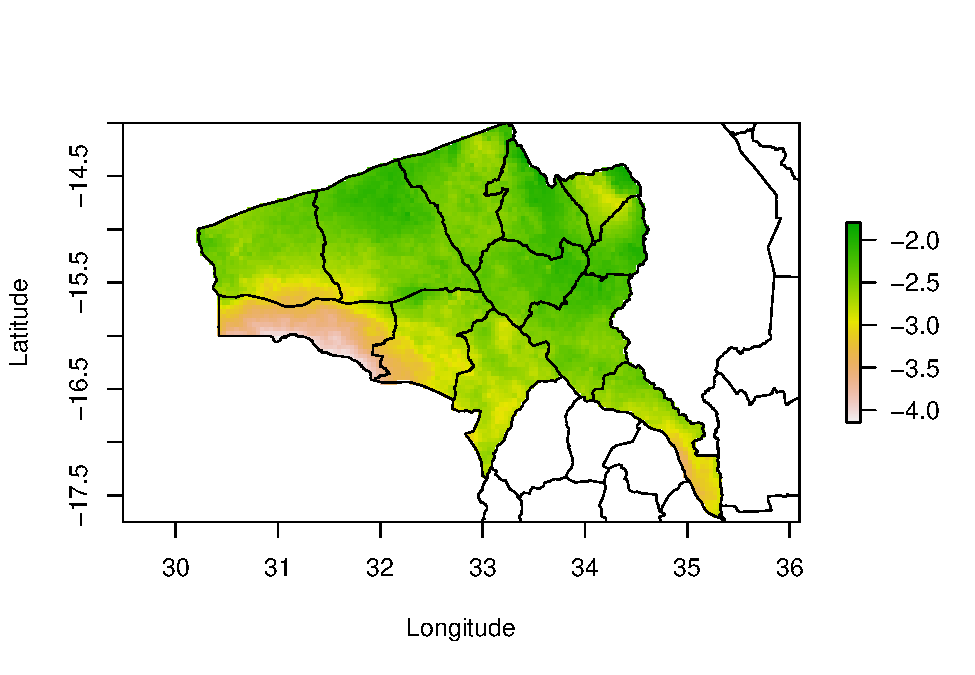
\includegraphics{Mozambique-NAP_files/figure-latex/ssp245-tete-1.pdf}

Fig. xx Mean temperature change (C) for Tete for 2021 -- 2040 compared to reference period 1971 -- 2000 for the medium emissions scenario (ssp245). BCC-CSM2-MR Model

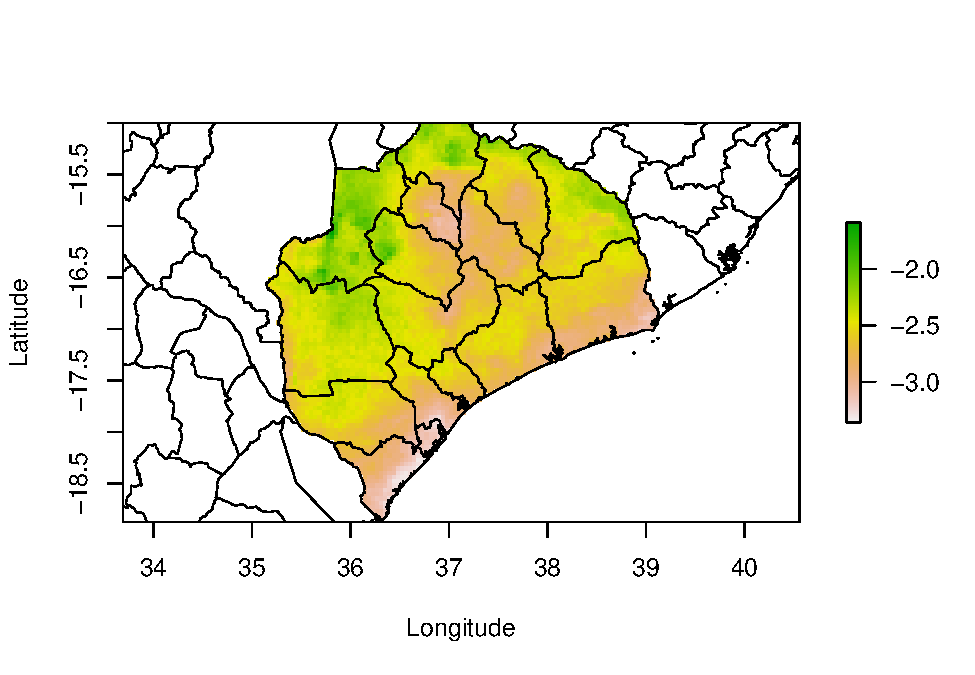
\includegraphics{Mozambique-NAP_files/figure-latex/ssp245-zambezia-1.pdf}

Fig. xx Mean temperature change (C) for Zambezia for 2021 -- 2040 compared to reference period 1971 -- 2000 for the medium emissions scenario (ssp245). BCC-CSM2-MR Model

\hypertarget{ssp585}{%
\subsubsection{ssp585}\label{ssp585}}

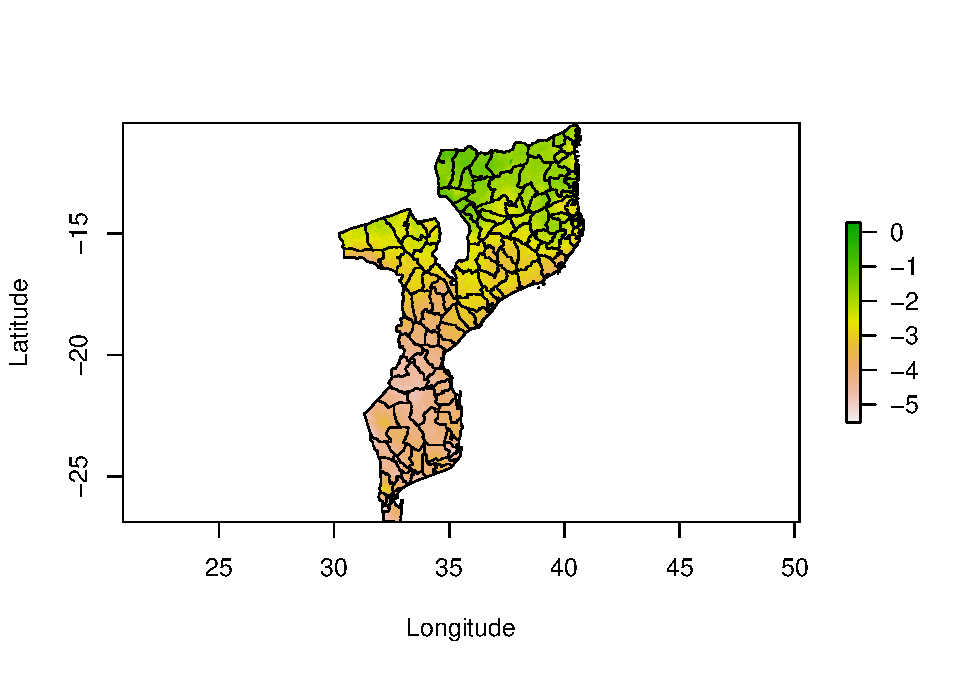
\includegraphics{Mozambique-NAP_files/figure-latex/ssp585-1.pdf}

Fig. 4b. Mean temperature change (C) for Mozambique for 2021 -- 2040 compared to reference period 1971 -- 2000 for the high emissions scenario (585). BCC-CSM2-MR Model.

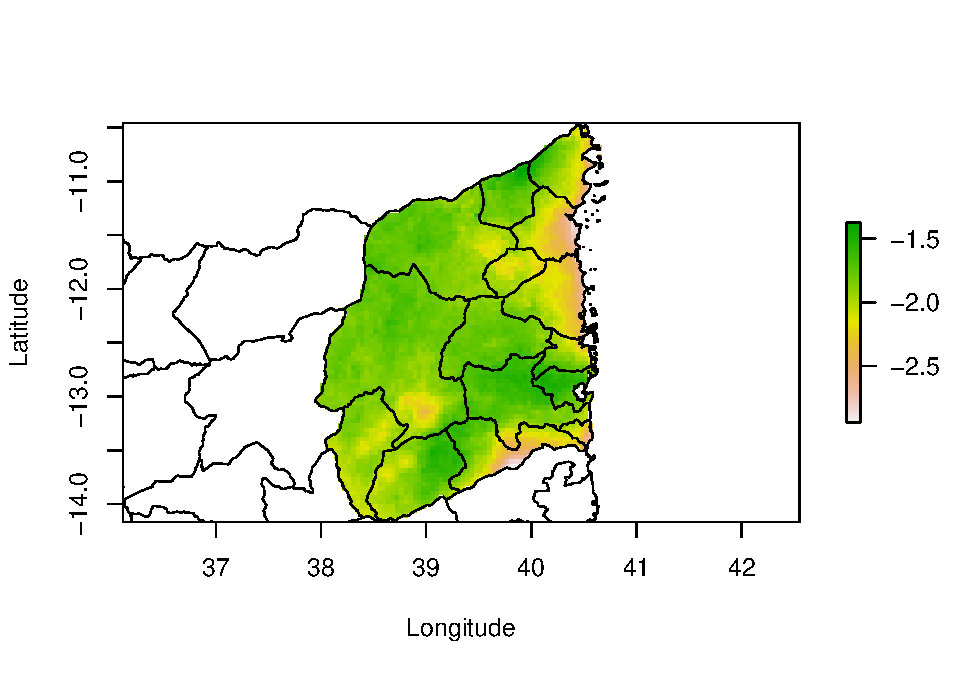
\includegraphics{Mozambique-NAP_files/figure-latex/ssp585-cabo-1.pdf}

Fig. 4b. Mean temperature change (C) for Cabo Delgado for 2020 -- 2040 compared to reference period 1971 -- 2000 for the high emissions scenario (585). BCC-CSM2-MR Model.

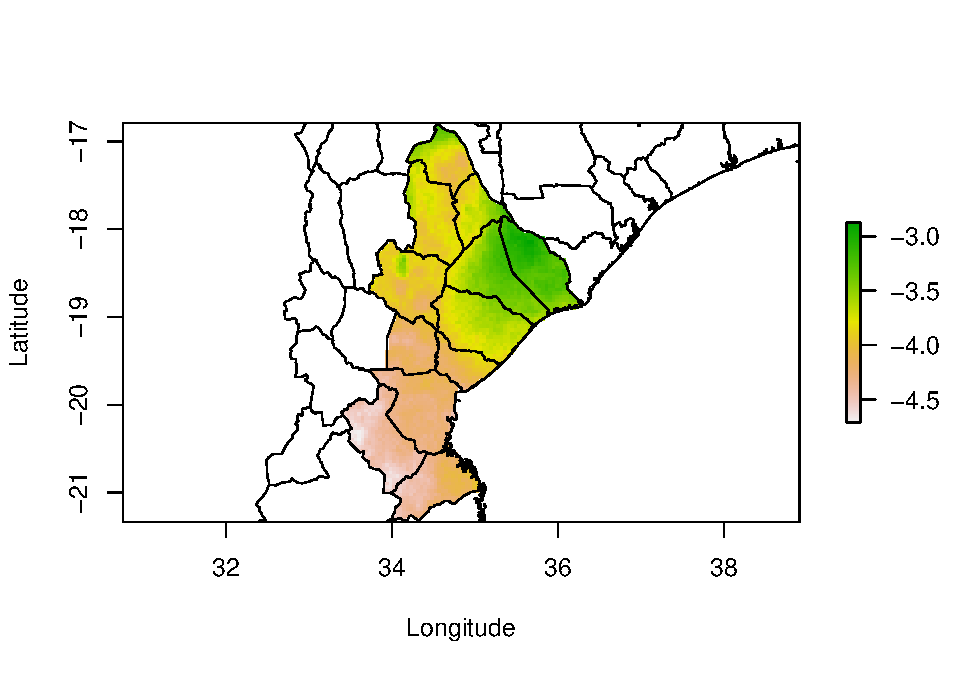
\includegraphics{Mozambique-NAP_files/figure-latex/ssp585-sofala-1.pdf}

Fig. 4b. Mean temperature change (C) for maputo for 2021 -- 2040 compared to reference period 1971 -- 2000 for the high emissions scenario (585). BCC-CSM2-MR Model.

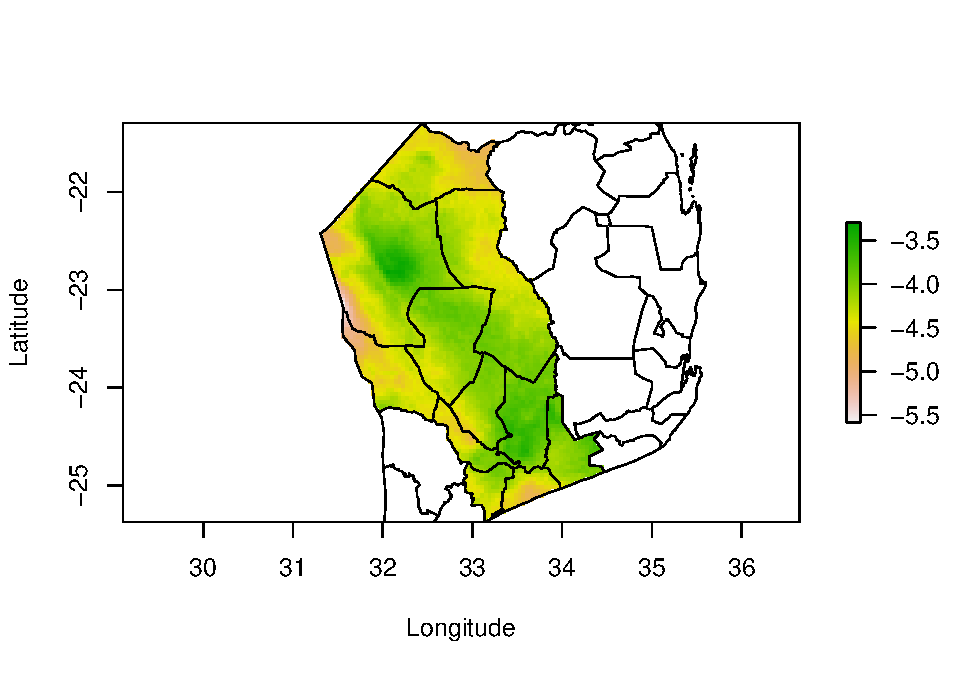
\includegraphics{Mozambique-NAP_files/figure-latex/ssp585-gaza-1.pdf}

Fig. xx Mean temperature change (C) for Gaza for 2021 -- 2040 compared to reference period 1971 -- 2000 for the high emissions scenario (ssp585). BCC-CSM2-MR Model

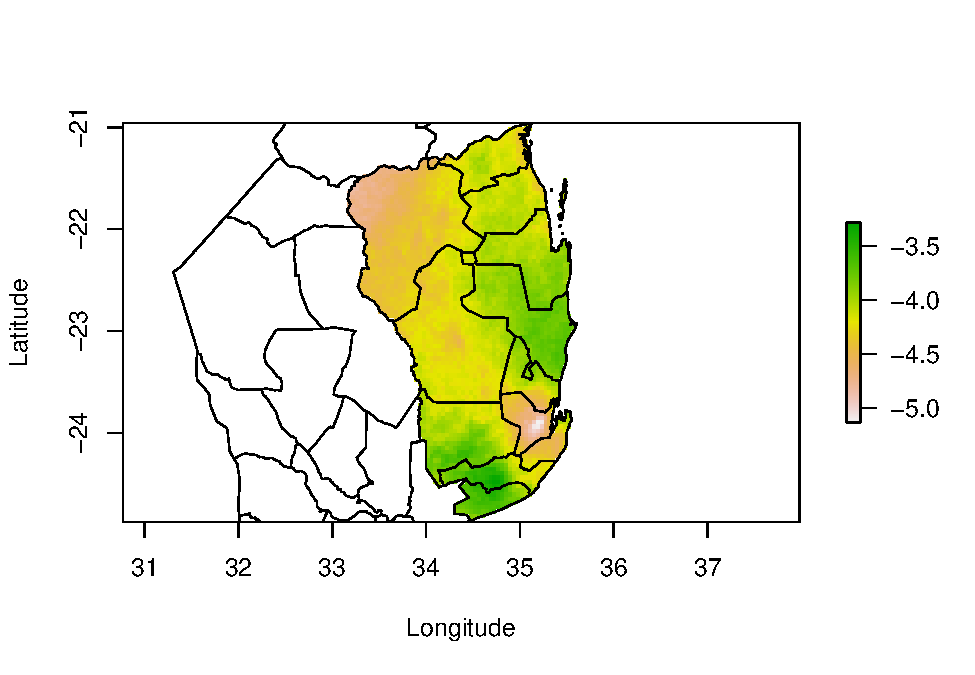
\includegraphics{Mozambique-NAP_files/figure-latex/ssp585-inbane-1.pdf}

Fig. xx Mean temperature change (C) for Inhambane for 2021 -- 2040 compared to reference period 1971 -- 2000 for the high emissions scenario (ssp585). BCC-CSM2-MR Model

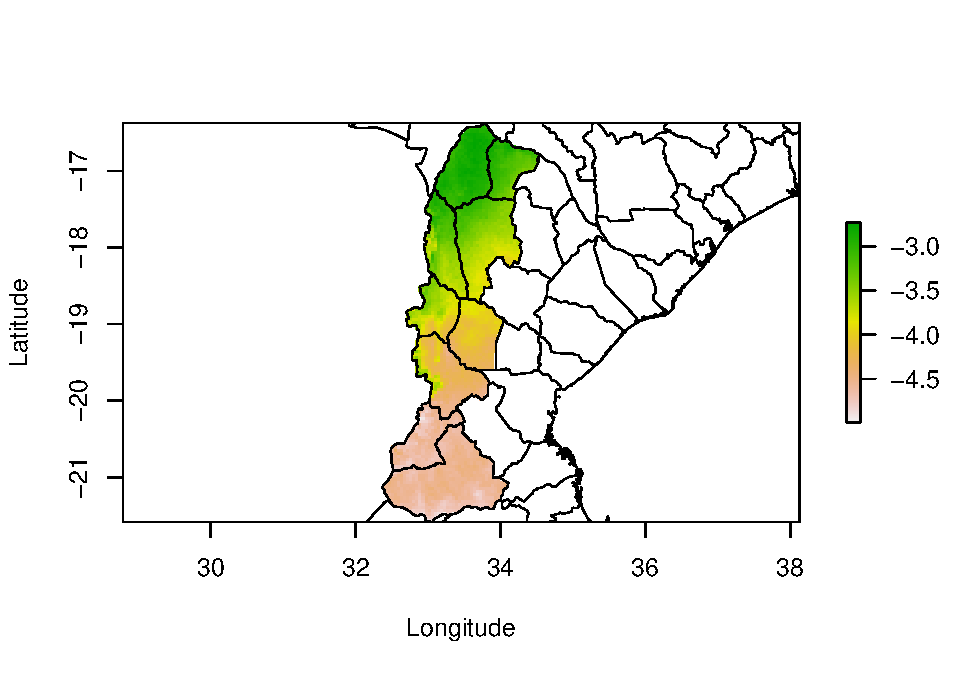
\includegraphics{Mozambique-NAP_files/figure-latex/ssp585-manica-1.pdf}

Fig. xx Mean temperature change (C) for Manica for 2021 -- 2040 compared to reference period 1971 -- 2000 for the high emissions scenario (ssp585). BCC-CSM2-MR Model

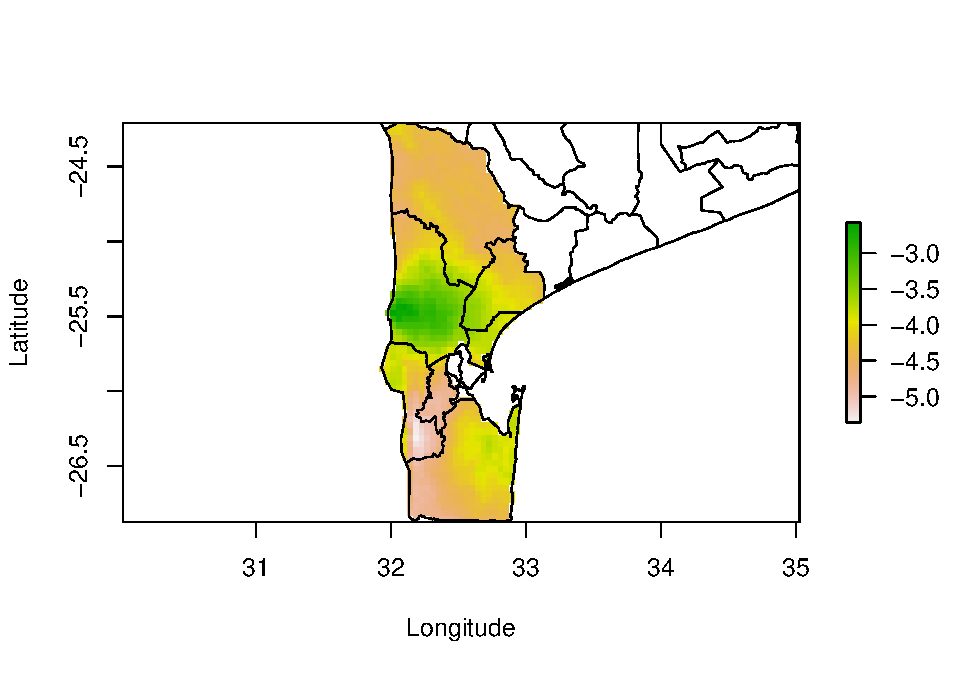
\includegraphics{Mozambique-NAP_files/figure-latex/ssp585-maputo-1.pdf}

Fig. xx Mean temperature change (C) for Maputo for 2021 -- 2040 compared to reference period 1971 -- 2000 for the high emissions scenario (ssp585). BCC-CSM2-MR Model

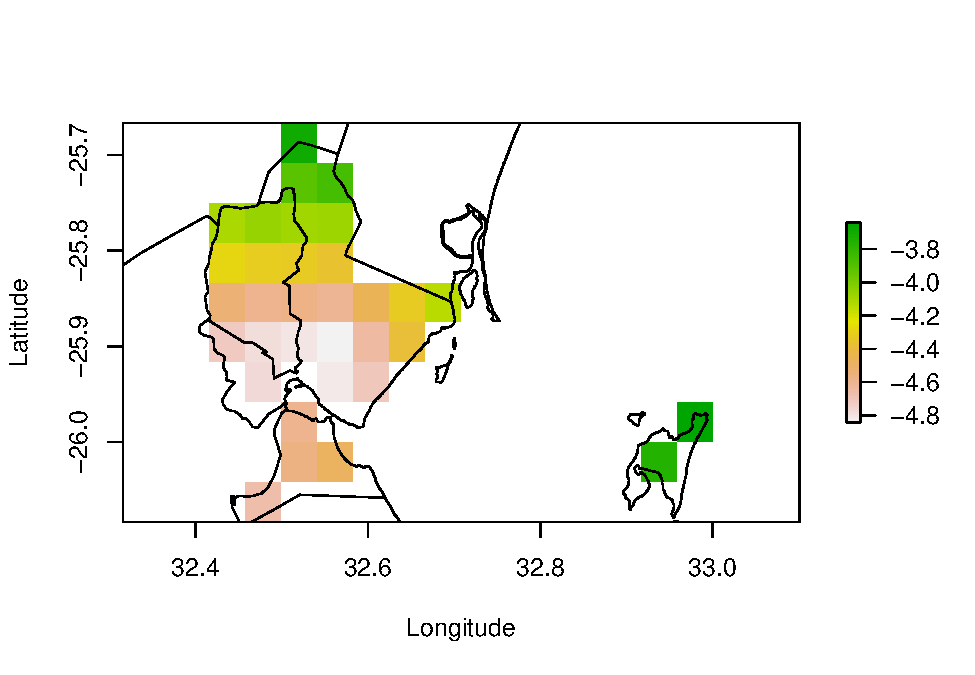
\includegraphics{Mozambique-NAP_files/figure-latex/ssp585-map.city-1.pdf}

Fig. xx Mean temperature change (C) for Maputo City for 2021 -- 2040 compared to reference period 1971 -- 2000 for the high emissions scenario (ssp585). BCC-CSM2-MR Model

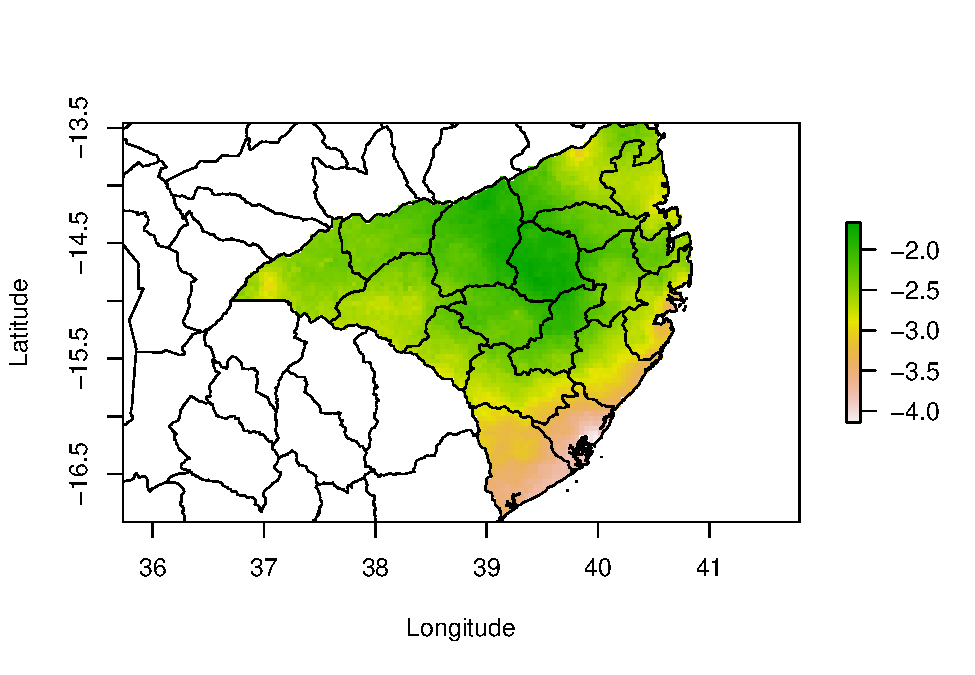
\includegraphics{Mozambique-NAP_files/figure-latex/ssp585-nampula-1.pdf}

Fig. xx Mean temperature change (C) for Nampula for 2021 -- 2040 compared to reference period 1971 -- 2000 for the high emissions scenario (ssp585). BCC-CSM2-MR Model

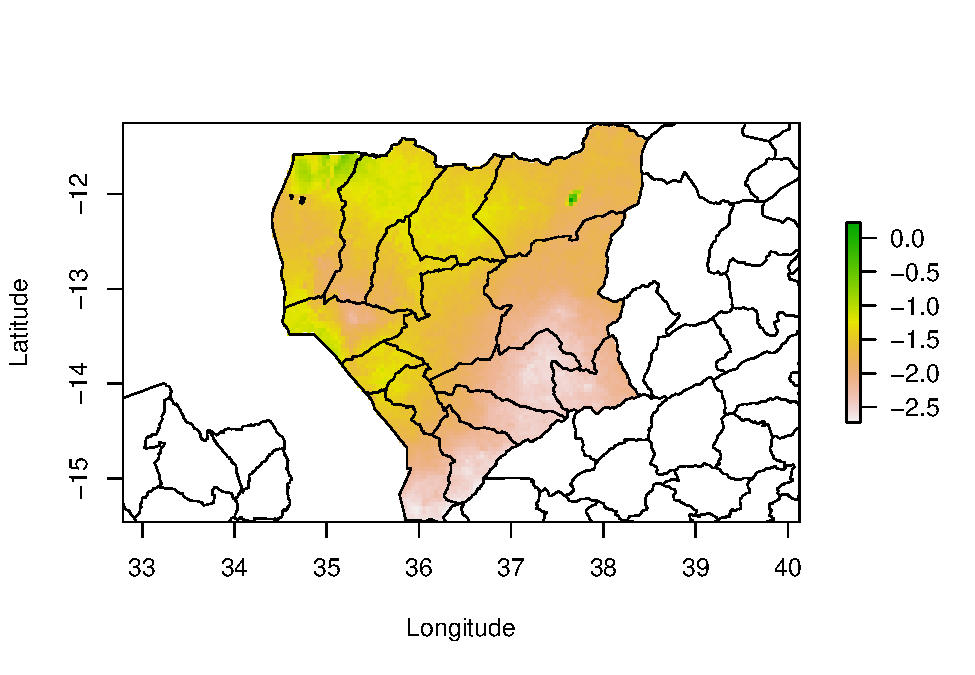
\includegraphics{Mozambique-NAP_files/figure-latex/ssp585-nassa-1.pdf}

Fig. xx Mean temperature change (C) for Nassa for 2021 -- 2040 compared to reference period 1971 -- 2000 for the high emissions scenario (ssp585). BCC-CSM2-MR Model

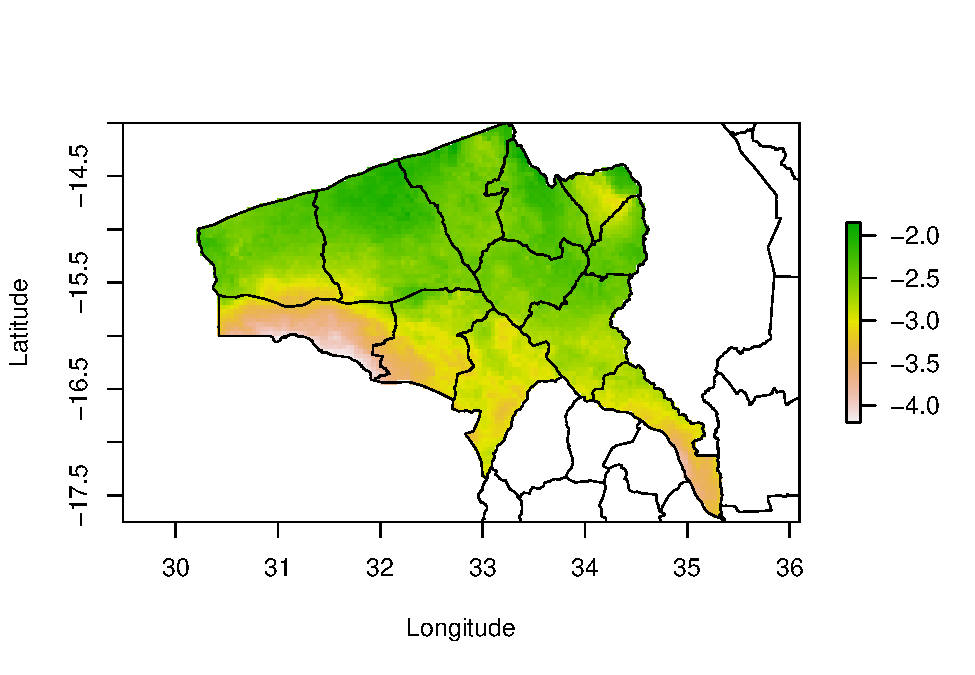
\includegraphics{Mozambique-NAP_files/figure-latex/ssp585-tete-1.pdf}

Fig. xx Mean temperature change (C) for Tete for 2021 -- 2040 compared to reference period 1971 -- 2000 for the high emissions scenario (ssp585). BCC-CSM2-MR Model

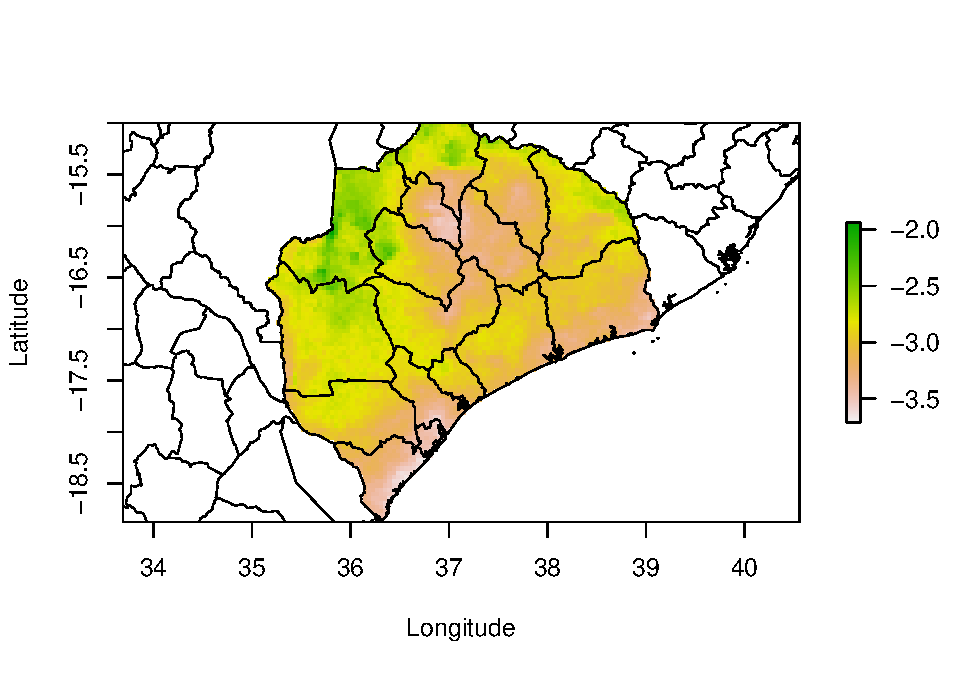
\includegraphics{Mozambique-NAP_files/figure-latex/ssp585-zambezia-1.pdf}

Fig. xx Mean temperature change (C) for Zambezia for 2021 -- 2040 compared to reference period 1971 -- 2000 for the high emissions scenario (ssp585). BCC-CSM2-MR Model

\hypertarget{projecuxe7uxf5es-futuras-da-precipitauxe7uxe3o}{%
\subsection{Projecções Futuras da Precipitação}\label{projecuxe7uxf5es-futuras-da-precipitauxe7uxe3o}}

As variações da precipitação não são tão claras como as da temperatura. A gama de projecções de precipitação resultantes de diferentes modelos é grande e abrange mudanças negativas e positivas. Há indicações de variações entre -15 a + 20 mm por mês, ou -15\% a + 34\% (Mcsweeney et al., 2010). Contudo, os modelos mostram mais coerência nas projecções sazonais, indicando redução das chuvas na estação seca, isto é, no período de Junho a Agosto (JJA) e de Setembro a Novembro (SON). Esta redução é compensada parcialmente pelo aumento das chuvas na estação chuvosa, no período de Dezembro a Fevereiro (DJF), com maior expressão no norte de Moçambique (Mcsweeney et al., 2010). Em geral, as projecções de precipitação não indicam mudanças substanciais na precipitação anual, mas sim na mudança dos padrões de precipitação (Figura 1.11).

\begin{figure}
\centering
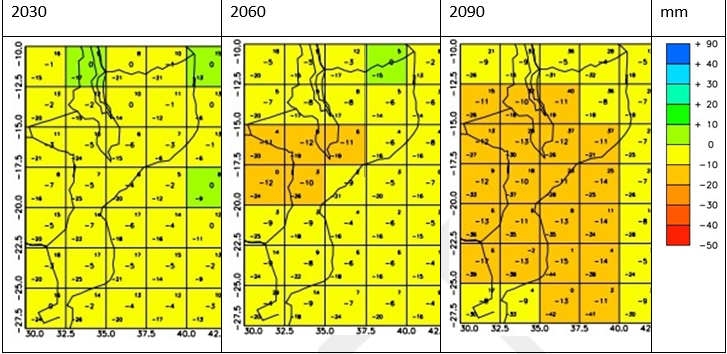
\includegraphics{images/padroes especiais.png}
\caption{Figura 1.11: Padrões espaciais das médias mensais de precipitação no período de setembro a novembro projectada para os anos 2030, 2060 e 2090 (Adaptado de Mcsweeney et al., 2010).}
\end{figure}

\hypertarget{ssp126}{%
\subsubsection{ssp126}\label{ssp126}}

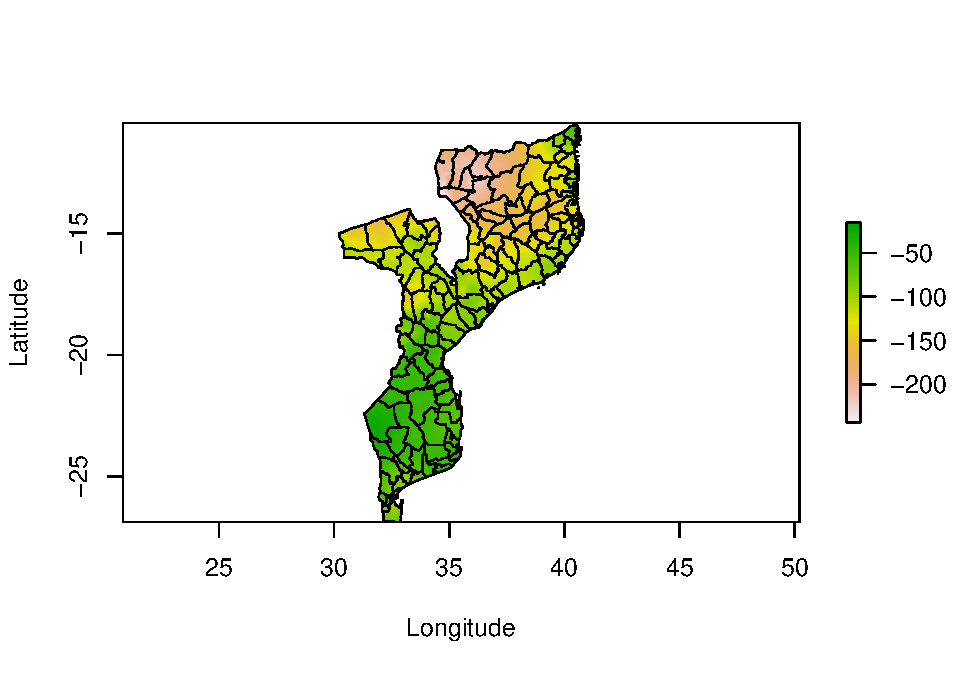
\includegraphics{Mozambique-NAP_files/figure-latex/pr126-national-1.pdf}

Fig. 5a. Precipitation (annual mean) for Mozambique for 2020 -- 2040 compared to reference period 1971 -- 2000 for the high emissions scenario (SSP585). BCC-CSM2-MR Model.

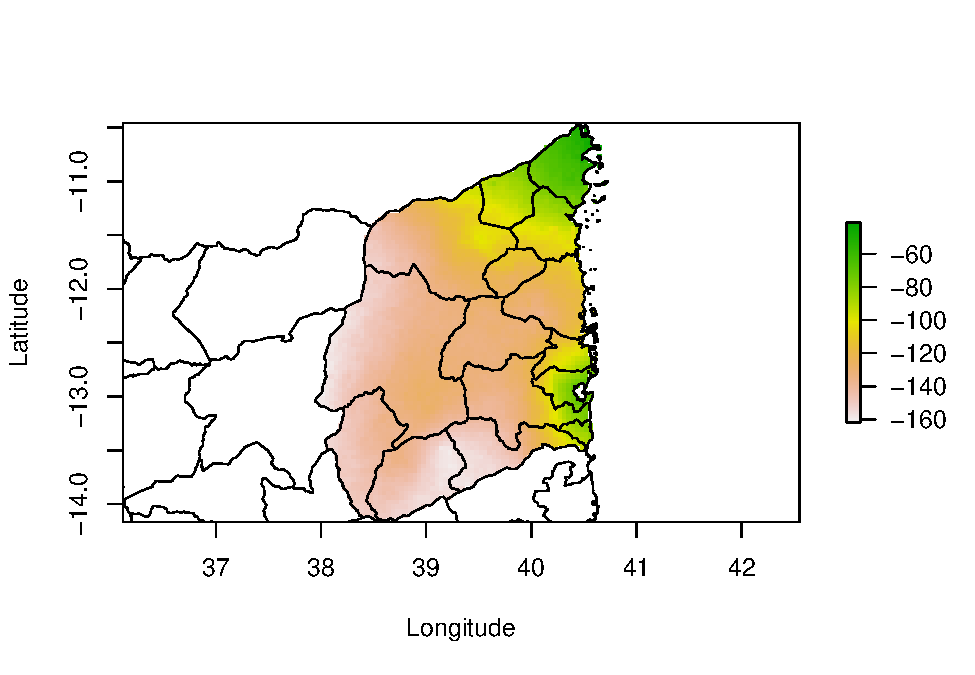
\includegraphics{Mozambique-NAP_files/figure-latex/pr126-cabo-1.pdf}

Fig. 4b. Mean precipitation change (C) for Cabo Delgado for 2020 -- 2040 compared to reference period 1971 -- 2000 for the low emissions scenario (ssp126). BCC-CSM2-MR Model.

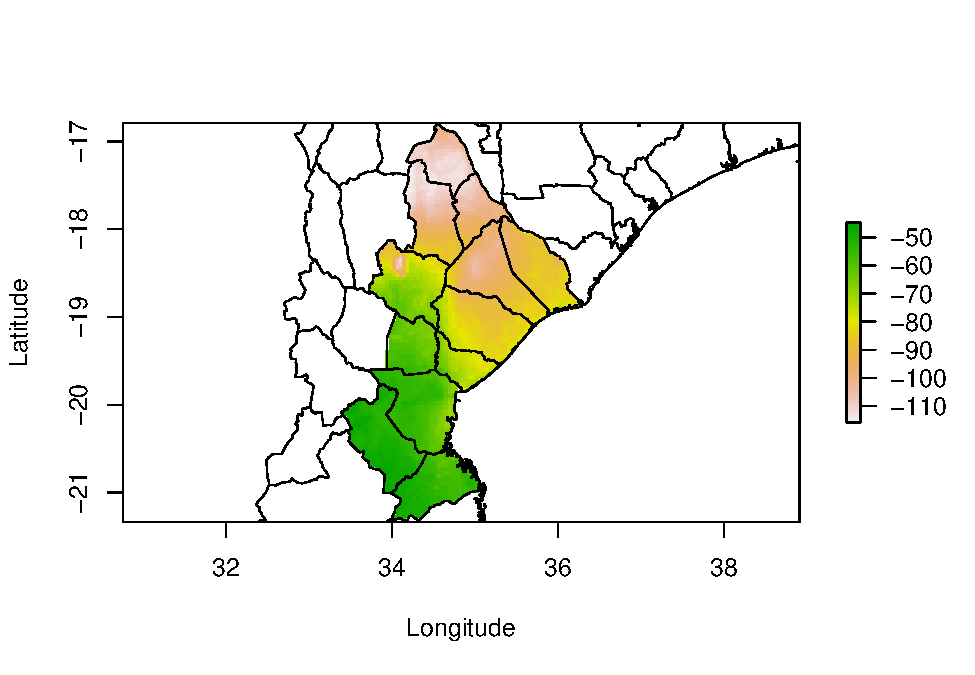
\includegraphics{Mozambique-NAP_files/figure-latex/pr126-sofala-1.pdf}

Fig. 4b. Mean precipitation change (C) for Sofala for 2021 -- 2040 compared to reference period 1971 -- 2000 for the low emissions scenario (ssp126). BCC-CSM2-MR Model.

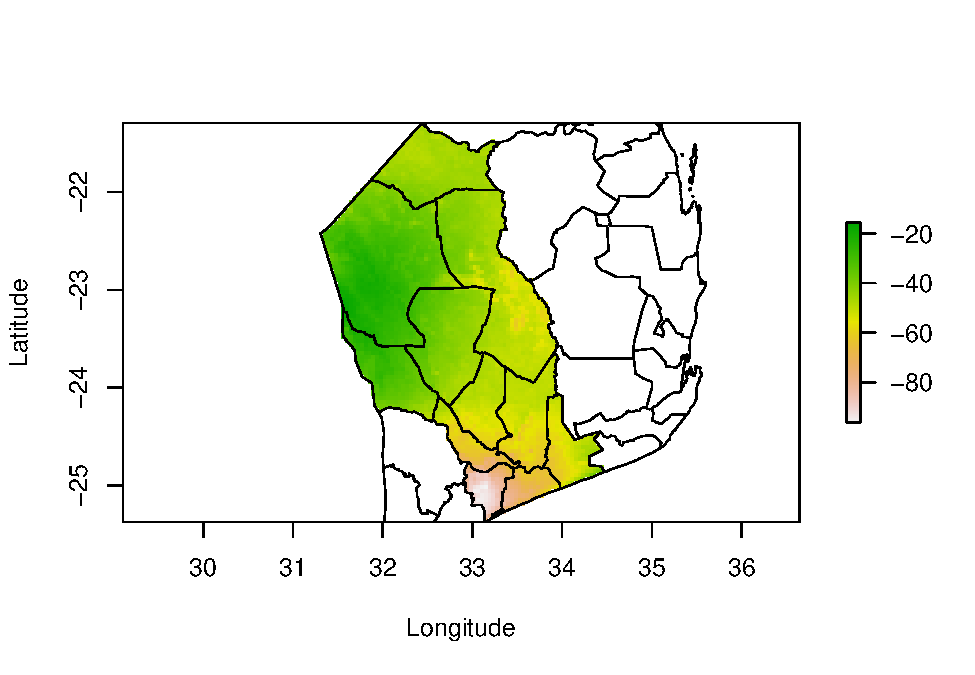
\includegraphics{Mozambique-NAP_files/figure-latex/pr126-gaza-1.pdf}

Fig. xx Mean precipitation change (C) for Gaza for 2021 -- 2040 compared to reference period 1971 -- 2000 for the low emissions scenario (ssp126). BCC-CSM2-MR Model

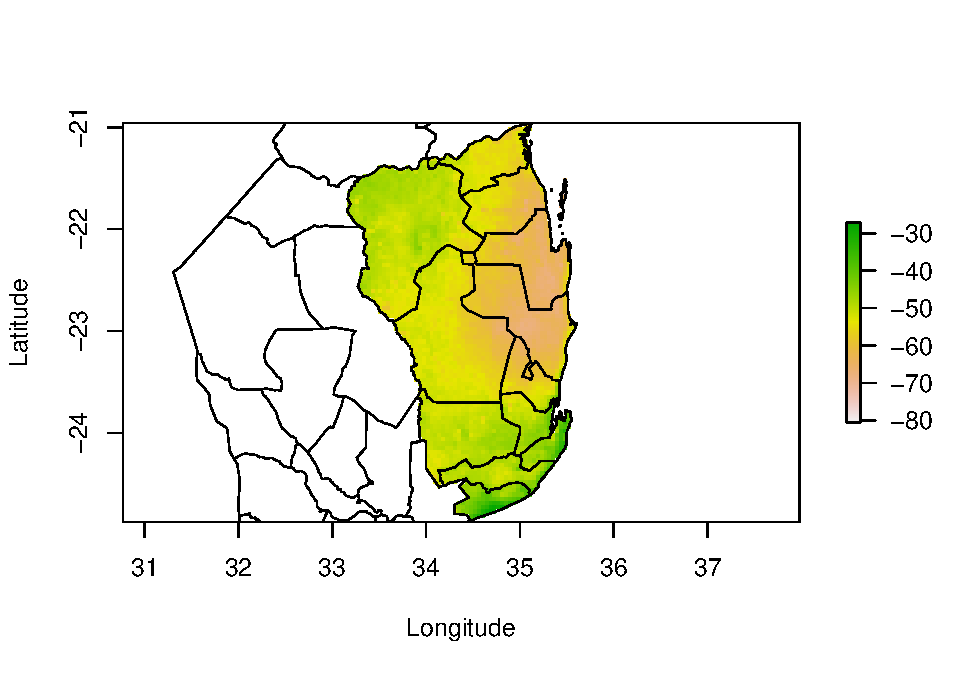
\includegraphics{Mozambique-NAP_files/figure-latex/pr126-inbane-1.pdf}

Fig. xx Mean precipitation change (C) for Inhambane for 2021 -- 2040 compared to reference period 1971 -- 2000 for the low emissions scenario (ssp126). BCC-CSM2-MR Model

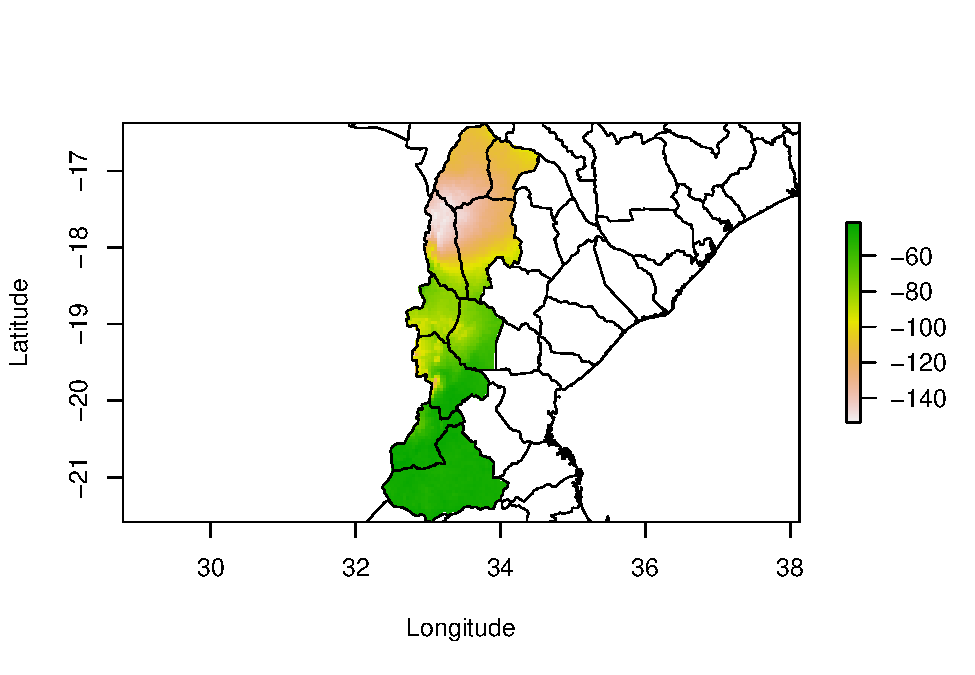
\includegraphics{Mozambique-NAP_files/figure-latex/pr126-manica-1.pdf}

Fig. xx Mean precipitation change (C) for Manica for 2021 -- 2040 compared to reference period 1971 -- 2000 for the low emissions scenario (ssp126). BCC-CSM2-MR Model

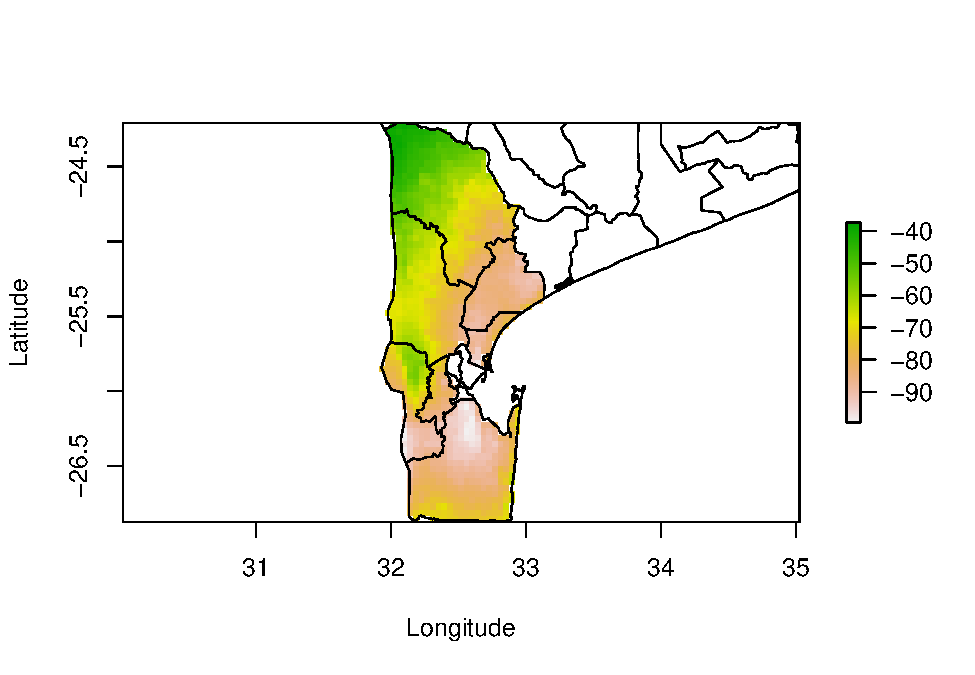
\includegraphics{Mozambique-NAP_files/figure-latex/pr126-maputo-1.pdf}

Fig. xx Mean precipitation change (C) for Maputo for 2021 -- 2040 compared to reference period 1971 -- 2000 for the low emissions scenario (ssp126). BCC-CSM2-MR Model

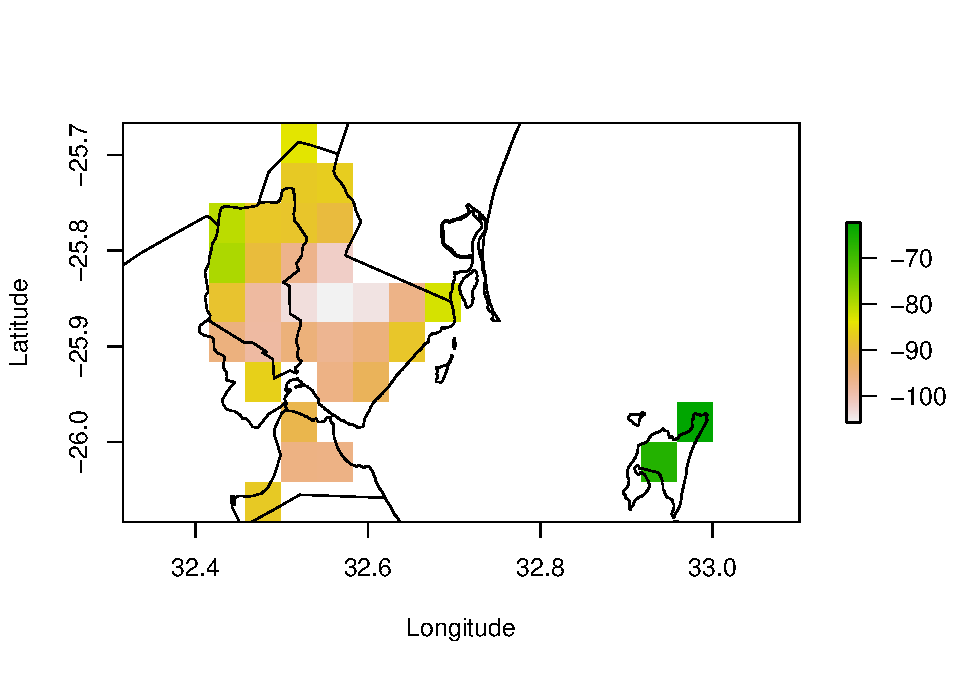
\includegraphics{Mozambique-NAP_files/figure-latex/pr126-map.city-1.pdf}

Fig. xx Mean precipitation change (C) for Maputo City for 2021 -- 2040 compared to reference period 1971 -- 2000 for the low emissions scenario (ssp126). BCC-CSM2-MR Model

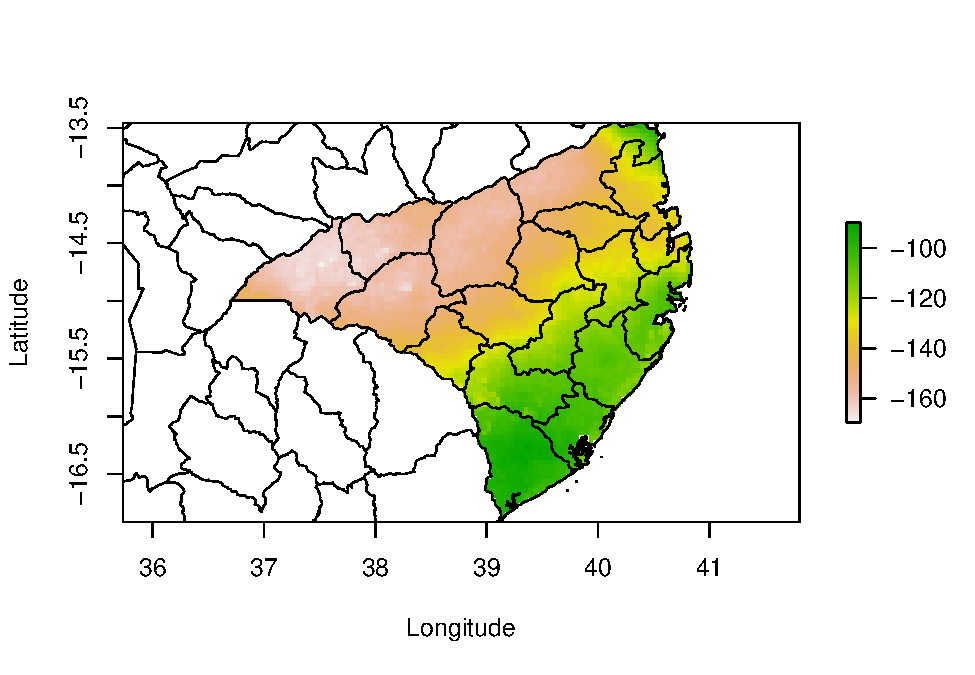
\includegraphics{Mozambique-NAP_files/figure-latex/pr126-nampula-1.pdf}

Fig. xx Mean precipitation change (C) for Nampula for 2021 -- 2040 compared to reference period 1971 -- 2000 for the low emissions scenario (ssp126). BCC-CSM2-MR Model

\includegraphics{Mozambique-NAP_files/figure-latex/pr126-nassa-1.pdf}

Fig. xx Mean precipitation change (C) for Nassa for 2021 -- 2040 compared to reference period 1971 -- 2000 for the low emissions scenario (ssp126). BCC-CSM2-MR Model

\includegraphics{Mozambique-NAP_files/figure-latex/pr126-tete-1.pdf}

Fig. xx Mean precipitation change (C) for Tete for 2021 -- 2040 compared to reference period 1971 -- 2000 for the low emissions scenario (ssp126). BCC-CSM2-MR Model

\includegraphics{Mozambique-NAP_files/figure-latex/pr126-zambezia-1.pdf}

Fig. xx Mean precipitation change (C) for Zambezia for 2021 -- 2040 compared to reference period 1971 -- 2000 for the low emissions scenario (ssp126). BCC-CSM2-MR Model

\hypertarget{ssp245-1}{%
\subsubsection{ssp245}\label{ssp245-1}}

\includegraphics{Mozambique-NAP_files/figure-latex/pr245-national-1.pdf}

Fig. 5b. Precipitation (annual mean) for Mozambique for 2020 -- 2040 compared to reference period 1971 -- 2000 for the medium emissions scenario (SSP245). BCC-CSM2-MR Model.

\includegraphics{Mozambique-NAP_files/figure-latex/pr245-cabo-1.pdf}

Fig. 4b. Mean precipitation change (C) for Cabo Delgado for 2020 -- 2040 compared to reference period 1971 -- 2000 for the medium emissions scenario (ssp245). BCC-CSM2-MR Model.

\includegraphics{Mozambique-NAP_files/figure-latex/pr245-sofala-1.pdf}

Fig. 4b. Mean precipitation change (C) for maputo for 2021 -- 2040 compared to reference period 1971 -- 2000 for the medium emissions scenario (ssp245). BCC-CSM2-MR Model.

\includegraphics{Mozambique-NAP_files/figure-latex/pr245-gaza-1.pdf}

Fig. xx Mean precipitation change (C) for Gaza for 2021 -- 2040 compared to reference period 1971 -- 2000 for the medium emissions scenario (ssp245). BCC-CSM2-MR Model

\includegraphics{Mozambique-NAP_files/figure-latex/pr245-inbane-1.pdf}

Fig. xx Mean precipitation change (C) for Inhambane for 2021 -- 2040 compared to reference period 1971 -- 2000 for the medium emissions scenario (ssp245). BCC-CSM2-MR Model

\includegraphics{Mozambique-NAP_files/figure-latex/pr245-manica-1.pdf}

Fig. xx Mean precipitation change (C) for Manica for 2021 -- 2040 compared to reference period 1971 -- 2000 for the medium emissions scenario (ssp245). BCC-CSM2-MR Model

\includegraphics{Mozambique-NAP_files/figure-latex/pr245-maputo-1.pdf}

Fig. xx Mean precipitation change (C) for Maputo for 2021 -- 2040 compared to reference period 1971 -- 2000 for the medium emissions scenario (ssp245). BCC-CSM2-MR Model

\includegraphics{Mozambique-NAP_files/figure-latex/pr245-map.city-1.pdf}

Fig. xx Mean precipitation change (C) for Maputo City for 2021 -- 2040 compared to reference period 1971 -- 2000 for the medium emissions scenario (ssp245). BCC-CSM2-MR Model

\includegraphics{Mozambique-NAP_files/figure-latex/pr245-nampula-1.pdf}

Fig. xx Mean precipitation change (C) for Nampula for 2021 -- 2040 compared to reference period 1971 -- 2000 for the medium emissions scenario (ssp245). BCC-CSM2-MR Model

\includegraphics{Mozambique-NAP_files/figure-latex/pr245-nassa-1.pdf}

Fig. xx Mean precipitation change (C) for Nassa for 2021 -- 2040 compared to reference period 1971 -- 2000 for the medium emissions scenario (ssp245). BCC-CSM2-MR Model

\includegraphics{Mozambique-NAP_files/figure-latex/pr245-tete-1.pdf}

Fig. xx Mean precipitation change (C) for Tete for 2021 -- 2040 compared to reference period 1971 -- 2000 for the medium emissions scenario (ssp245). BCC-CSM2-MR Model

\includegraphics{Mozambique-NAP_files/figure-latex/pr245-zambezia-1.pdf}

Fig. xx Mean precipitation change (C) for Zambezia for 2021 -- 2040 compared to reference period 1971 -- 2000 for the medium emissions scenario (ssp245). BCC-CSM2-MR Model

\hypertarget{ssp585-1}{%
\subsubsection{ssp585}\label{ssp585-1}}

\includegraphics{Mozambique-NAP_files/figure-latex/pr-585-national-1.pdf}

Fig. 5c. Precipitation (annual mean) for Mozambique for 2020 -- 2040 compared to reference period 1971 -- 2000 for the high emissions scenario (SSP585). BCC-CSM2-MR Model.

\includegraphics{Mozambique-NAP_files/figure-latex/pr585-cabo-1.pdf}

Fig. 4b. Mean precipitation change (C) for Cabo Delgado for 2020 -- 2040 compared to reference period 1971 -- 2000 for the high emissions scenario (ssp585). BCC-CSM2-MR Model.

\includegraphics{Mozambique-NAP_files/figure-latex/pr585-sofala-1.pdf}

Fig. 4b. Mean precipitation change (C) for maputo for 2021 -- 2040 compared to reference period 1971 -- 2000 for the high emissions scenario (ssp585). BCC-CSM2-MR Model.

\includegraphics{Mozambique-NAP_files/figure-latex/pr585-gaza-1.pdf}

Fig. xx Mean precipitation change (C) for Gaza for 2021 -- 2040 compared to reference period 1971 -- 2000 for the high emissions scenario (ssp585). BCC-CSM2-MR Model

\includegraphics{Mozambique-NAP_files/figure-latex/pr585-inbane-1.pdf}

Fig. xx Mean precipitation change (C) for Inhambane for 2021 -- 2040 compared to reference period 1971 -- 2000 for the high emissions scenario (ssp585). BCC-CSM2-MR Model

\includegraphics{Mozambique-NAP_files/figure-latex/pr585-manica-1.pdf}

Fig. xx Mean precipitation change (C) for Manica for 2021 -- 2040 compared to reference period 1971 -- 2000 for the high emissions scenario (ssp585). BCC-CSM2-MR Model

\includegraphics{Mozambique-NAP_files/figure-latex/pr585-maputo-1.pdf}

Fig. xx Mean precipitation change (C) for Maputo for 2021 -- 2040 compared to reference period 1971 -- 2000 for the high emissions scenario (ssp585). BCC-CSM2-MR Model

\includegraphics{Mozambique-NAP_files/figure-latex/pr585-map.city-1.pdf}

Fig. xx Mean precipitation change (C) for Maputo City for 2021 -- 2040 compared to reference period 1971 -- 2000 for the high emissions scenario (ssp585). BCC-CSM2-MR Model

\includegraphics{Mozambique-NAP_files/figure-latex/pr585-nampula-1.pdf}

Fig. xx Mean precipitation change (C) for Nampula for 2021 -- 2040 compared to reference period 1971 -- 2000 for the high emissions scenario (ssp585). BCC-CSM2-MR Model

\includegraphics{Mozambique-NAP_files/figure-latex/pr585-nassa-1.pdf}

Fig. xx Mean precipitation change (C) for Nassa for 2021 -- 2040 compared to reference period 1971 -- 2000 for the high emissions scenario (ssp585). BCC-CSM2-MR Model

\includegraphics{Mozambique-NAP_files/figure-latex/pr585-tete-1.pdf}

Fig. xx Mean precipitation change (C) for Tete for 2021 -- 2040 compared to reference period 1971 -- 2000 for the high emissions scenario (ssp585). BCC-CSM2-MR Model

\includegraphics{Mozambique-NAP_files/figure-latex/pr585-zambezia-1.pdf}

Fig. xx Mean precipitation change (C) for Zambezia for 2021 -- 2040 compared to reference period 1971 -- 2000 for the high emissions scenario (ssp585). BCC-CSM2-MR Model

\hypertarget{climate-change-adaptation-assessment}{%
\section{Climate change adaptation assessment}\label{climate-change-adaptation-assessment}}

\#\#\#\#\#\#\#\#\#\#\#\#\#\#\#\#\#\#\#\#\#\#\#3table\#\#\#\#\#\#\#\#\#\#\#\#\#\#\#

\#\#\#\#\#\#\#\#\#\#\#\#\#\#\#\#\#\#\#\#\#tablesssssssssssssss

\hypertarget{national-adaptation-priorities}{%
\chapter{National adaptation priorities}\label{national-adaptation-priorities}}

\begin{itemize}
\tightlist
\item
  Aumentar a
\end{itemize}

(To address the key impacts, vulnerabilities and risks covering the economy, environment and the social including gender, covering all adaptation needs including those being addressed already -- the national adaptation portfolio/the national adaptation effort)
a. NAPA
b. National Strategy of Gender Environment and Climate Change\\
c.~National Determined Contributions (NDC)
d.~Local Adaptations Plans (Covering 106 districts out of 152 districts)
e. National Strategy of Basic Social Security
f.~Strategic Plan of the Health Sector that include Climate Change\\
g. Action Plan for the Fishery Sector for Climate Change
h. Action Plan for Climate Resilient Agriculture
Climate change adaptation implementation strategy including costs
a. National climate change adaptation Strategy: umbrella programme

\begin{enumerate}
\def\labelenumi{\alph{enumi}.}
\setcounter{enumi}{1}
\item
  Projects and programmes to address key risks for the country
  \#\#\#\#\#\#\#\#\#\#\#\#\#\#\#\#\#table\#\#\#\#\#\#\#\#\#\#\#\#\#\#\#3
\item
  Essential cross-cutting projects/programmes
\item
  Creating an effective adaptation process and system (mainstreaming/integration, policies, governance, etc.)
\end{enumerate}

\begin{enumerate}
\def\labelenumi{\roman{enumi}.}
\setcounter{enumi}{1}
\tightlist
\item
  Climate information services and early warnings systems, systematic observations
\end{enumerate}

O Instituto Nacional de Meteorologia de Moçambique (INAM) é a principal instituição responsável pela colecta, tratamento e arquivo de dados meteorológicos e climáticos em Moçambique. O INAM faz a colecta de dados meteorológicos a partir sua rede de estações meteorológicas que são operadas em todo o país. O INAM tem mandato para fornecer informações meteorológicas para apoiar o planeamento, bem como para fornecer aviso prévio, sempre que necessário, para minimizar riscos de vida e bens. O INAM fornece várias previsões e produtos meteorológicos diferentes ao longo do ano, incluindo, entre outros, previsões meteorológicas diárias e sazonais, observações meteorológicas e climáticas e produtos especializados para os sectores da aviação e marinha. As previsões públicas emitidas pelo INAM incluem três previsões diárias - duas previsões de 24 horas emitidas pela manhã e tarde, respectivamente, mais uma previsão de `quatro dias' emitida todas as manhãs. Além das previsões diárias transmitidas pela Comunicação Social, como notícias nacionais e a página do INAM, o Instituto prepara previsões agrícolas sazonais para cada província que são apresentadas no início da temporada agrícola, geralmente em Setembro (ou seja, nas semanas anteriores ao início da a estação das chuvas, quando os agricultores começam a preparar suas terras).

\textbf{Observações hidrológicas}

As Administrações Regionais de Água (ARAs - Sul, Centro, Centro Norte, Norte e Zambeze) e a Direcção Nacional de Gestão dos Recursos Hídricos (DNGRH) são instituições sob tutela do Ministério das Obras Públicas, Habitação e Recursos Hídricos (MOPHRH) que fazem a provisão de dados hidrológicos e de precipitação ao mesmo tempo que garantem os serviços de informação hidrológica para apoiar o planeamento e gestão de recursos hídricos na monitoria e análise das alterações climáticas, gestão ambiental e planeamento, operações hidroeléctricas e barragens, planeamento de sistemas de irrigação e aviso prévio de desastres relacionados com a água. Os principais temas dos serviços hidrológicos são:
(i) Planeamento de recursos hídricos e alocação;
(ii) Gestão operacional de infra-estruturas hidráulicas;
(iii) Gestão ambiental;
(iv) Avaliação de risco de inundação, Planeamento de Redução de Risco e Controlo de Cheias;
(v) Gestão de Seca no sistema de aviso prévio;
(vi) Gestão da poluição;
(vii) Mudança climática;
(viii) Gestão da irrigação.

\textbf{Observações agro-climáticas}

O Instituto de Investigação Agrária de Moçambique (IIAM), subordinada ao MASA, é a principal instituição de pesquisa agrícola de Moçambique. O IIAM está focalizado, principalmente, em pesquisa e desenvolvimento para apoiar a produtividade e eficiência do sector agrícola de Moçambique, particularmente, através da geração de produtos de pesquisa local e oportuna para informar às partes interessadas em toda a cadeia de valor agrícola. O IIAM também é responsável pela comunicação de informações técnicas pertinentes às partes interessadas relevantes para o sector agrícola, os decisores políticos do governo, os extensionistas e agricultores ao nível do campo. O foco da pesquisa do IIAM inclui ciências agronómicas, florestais e animais, sociologia rural e economia e agronegócios, que é realizado com o objectivo de fornecer orientação científica, técnica e administrativa ao MASA e a outras instituições públicas envolvidas no sector agrícola.

\textbf{Observações oceanográficas e monitorização do nível do mar}

O Instituto Nacional de Hidrografia e Navegação (INAHINA) é uma instituição tutelada pelo Ministro que superintende o sector dos Transportes Marítimos e é parte integrante do Ministério dos Transportes e Comunicações. A função principal do INAHINA é de facilitar a navegação segura nas águas costeiras e interiores do país, através de serviços hidrográficos, oceanográficos assim como instalação, reabilitação e manutenção de ajudas à navegação incluindo a calibração de agulhas magnéticas. A observação e monitorização do nível do mar faz parte de uma das suas atribuições no domínio da coordenação, cooperação, desenvolvimento e acompanhamento de actividades de investigação, estudos e trabalhos no domínio de Hidrografia, Cartografia Náutica, Oceanografia e Navegação. Estudos sobre elevação do nível do mar (SLR) vêm sendo realizados no INAHINA, INAM e ao nível da academia (p.~ex. UEM). Até agora, a avaliação realizada foi baseada em dados históricos medidos a partir de marégrafos e altimetria de satélites. Não obstante, um estudo conduzido pelo Instituto Nacional de Gestão de Calamidades (INGC, 2009) em parceria com instituições nacionais, regionais e internacionais fez uma avaliação, combinando a abordagem histórica e projecções climáticas da elevação do nível do mar usando cenários descritos no IPCC (2007) conhecidos como SRES . Dados observacionais mais actualizados e projecções de elevação do nível do mar (SLR) tendo em conta cenários mais recentes precisam de ser considerados para uma avaliação mais consistente.

\textbf{Observações de dados oceano-físico-biológicos e monitorização da ocorrência de recursos pesqueiros}

O Instituto Nacional de Investigação Pesqueira (IIP) é uma instituição pública subordinada ao Ministério do Mar, Águas Interiores e Pescas (MIMAIP) e que desenvolve trabalhos de investigação necessários ao conhecimento científico dos recursos pesqueiros das águas jurisdicionais moçambicanas tendo em vista a sua gestão, conservação e optimização da sua exploração. O IIP realiza cruzeiros de investigação pesqueira que permitem fazer a monitorização científica da ocorrência de recursos pesqueiros nas águas jurisdicionais moçambicanas e a medição dos parâmetros físicos e químicos do meio aquático, onde estes recursos habitam. A informação produzida através destes cruzeiros complementa os dados colhidos da actividade de pesca comercial e de subsistência é usada para avaliar o grau de exploração dos recursos com vista à gestão sustentável das pescarias. Através de cruzeiros de investigação são colhidos dados oceanográficos (CTD), dados de nutrientes, sedimentos, ventos, correntes, produtividade primária, mamíferos marinhos entre outros.

\textbf{Monitoria e vigilância em saúde pública}

O Observatório Nacional de Saúde (ONS) é uma instituição de âmbito nacional, subordinada ao Ministério da Saúde (MISAU). O ONS é centro nacional virtual concebido para a observação sistemática e fortalecimento do sistema de informação de saúde nacional. Com alicerces nas suas atribuições o ONS tem centrado as suas actividades, desde a sua criação em 2015, na análise de dados secundários com base na triangulação das fontes de dados de modo a ``informar para acção'' e assegurar o bem-estar da população. O ONS faz a integração: (i) de dados de diferentes fontes nomeadamente, de ministérios, instituições de pesquisa, ONGs, sociedade civil e instituições académicas; (ii) das funções de sistemas de informação, monitoria e vigilância em saúde já estabelecidos (por ex., CISM, INS). O ONS recomenda, sempre necessário, a produção de informação primária às entidades com este mandato. O ONS funciona através de plataformas multi-institucionais e multidisciplinares (HIV; Saúde da Mulher e Criança e Nutrição; Clima, Ambiente e Saúde; Mortalidade; Resistência Anti-microbiana; Sistemas de Saúde e PACE) que formam a rede de gestão do conhecimento. Através da plataforma de Clima, Ambiente e Saúde a instituição participa no Fórum Nacional de Antevisão Climática (FNAC), onde são produzidos, anualmente, mapas de risco de doenças sensíveis ao clima para a época chuvosa seguinte. Os principais indicadores usados na FNAC estão divididos em categorias nomeadamente: socio-demográficos, saúde -- programáticos, meteorológicos/climáticos e ambientais.

\textbf{Instituições utilizadoras de informações/dados observacionais}
A Tabela 5.8 mostra algumas instituições utilizadoras de informações/dados meteorológicas (os) e hidrológicas (os) entre outras (os) fornecidas (os) pelas instituições provedoras incluindo a sua finalidade e prioridade de uso.

Tabela 5.9: Papel das instituições utilizadoras de informações/dados meteorológicos (os) e hidrológicas (os) provenientes das instituições provedoras ( MOPHRH, 2016).

\#\#\#\#\#\#\#\#\#\#\#\#\#\#\#\#table\#\#\#\#\#\#\#\#\#\#\#\#\#\#\#\#\#\#

\hypertarget{estuxe1gio-actual-das-observauxe7uxf5es-em-mouxe7ambique}{%
\subsection{Estágio actual das observações em Moçambique}\label{estuxe1gio-actual-das-observauxe7uxf5es-em-mouxe7ambique}}

A rede de observações sistemáticas em Moçambique sofreu uma degradação progressiva depois da independência até aos anos 2000. Depois das cheias de 2000 houve investimentos nacionais e de parceiros internacionais que permitiram que actualmente a rede de observações esteja melhor do que o período anterior ao ano 2000, pese embora a sua representatividade espacial continua deficiente. Foram introduzidos neste período novos sistemas de observação automáticos, no entanto este processo não foi adequadamente acompanhado pela formação de pessoal qualificado para garantir sua manutenção, isto agravado pelo facto de os orçamentos não garantirem verbas suficientes para este exercício.\\
A melhoria dos serviços hidro-meteorológicos de Moçambique tem um potencial para aumentar a produtividade em sectores como a agricultura, pesca/marinha, energia hidroeléctrica, aviação, transporte rodoviário, planificação de infra-estruturas e na saúde. A informação hidro-meteorológica pode aumentar a produtividade desses sectores-chave da economia, fornecendo conhecimento que se pode traduzir num incremento da produção económica, através de uma melhor planificação e gestão adequada das infra-estruturas.
O papel dos serviços hidro-meteorológicos fornecidos pelas ARAs, a DNGRH e o INAM é reconhecido em vários pacotes legislativos, estratégias e políticas do Governo em Moçambique. Porém, a eficácia dos serviços no cumprimento do seu papel tem sido prejudicada por uma série de desafios caracterizada pela baixa densidade de estações pluviométricas (muitas necessitando de reabilitação e calibração) e diferentes níveis de soluções tecnológicas. Para qualquer das instituições não houve algum projecto sistemático de desenvolvimento da rede e, a localização das estações limita-se às sedes provinciais e distritais, bem como locais estratégicos, como aeroportos, postos experimentais agronómicos e partes da costa. Não obstante, a DNGRH e O INAM estão a liderar a implementação de um estudo de optimização da rede e serviços hidro-meteorológicos (MOPHRH, 2016), com o objectivo de desenhar intervenções necessárias que levarão à sua melhoria do seu funcionamento no país.

\textbf{Rede de observações hidrológicas}

Segundo os dados hidrológicos utilizados e fornecidos pelas 5 Administrações de Águas (ARAs) e confirmados pela base de dados central da DNGRH e analisados no relatório do estudo realizado pela empresa de consultoria SOLOMON durante a fase de diagnóstico dos serviços hidro-meteorológicos (MOPHRH, 2016), existe um total de 116 estações operacionais pertencentes aquelas entidades (Figura 5.2). Segundo este relatório, as observações hidrológicas colhidas a partir das estações hidrométricas das ARAs e DNGRH cobrem o período de 1930 a 2014, com particular destaque para o período de 1942 a 1981, onde o número de estações operacionais aumentou significativamente.

\begin{figure}
\centering
\includegraphics{images/hidrometricas_operacionais.png}
\caption{Figura 5.3: Distribuição espacial das estações hidrométricas operacionais e não operacionais (vede o mapa) e o número das estações operacionais (vede a tabela) na rede de monitoramento de caudais pela DNGRH e ARAs (MOPHRH, 2016).}
\end{figure}

Na rede de monitoramento de dados de precipitação foi constatada a existência de um total de 322 estações operacionais pertencentes a DNGRH e ARAs (Figura 5.3).

\begin{figure}
\centering
\includegraphics{images/pluviometricas_operacionais.png}
\caption{Figura 5.4: Distribuição espacial das estações pluviométricas operacionais e não operacionais (viz.~o mapa) e o número das estações pluviométricas operacionais (viz.~a tabela) na rede de monitoramento de precipitação pela DNGRH e ARAs (MOPHRH, 2016).}
\end{figure}

\textbf{Rede de observações meteorológicas e climáticas}
O INAM opera a principal rede de observações meteorológicas e climáticas do país. Os mapas abaixo (Figura 5.4) e a Tabela 5.8 e ilustram a evolução da rede com o tempo, usando como referência os anos 1975, 2000, 2011 e 2018 e a sua distribuição espacial. Como se pode notar entre 1975 e 2000 houve uma queda geral acentuada da rede nacional de observações gerida pelo INAM. Entre 2000 e 2011 houve progresso com aumento significativo das estações sinópticas e instalação de dois radares tempo, modernos, como resultado de investimentos significativos mobilizados em resposta às devastadoras cheias do ano 2000. Entre 2011 e 2018 houve um incremento mais significativo dos vários tipos de estações da rede de observação do INAM.

\begin{figure}
\centering
\includegraphics{images/estacoes_INAM.png}
\caption{Figura 5.5: Distribuição espacial das redes de estações do INAM (viz.~o mapa) e o número das estações sinópticas, climatológicas, agro-meteorológicos, aerológicas e de radar (INAM, 2016).}
\end{figure}

Tabela 5.10: Número das estações sinópticas, climatológicas e agro-climáticas operacionais e não operacionais do INAM

\#\#\#\#\#\#\#\#\#\#\#\#\#\#\#\#\#\#table\#\#\#\#\#\#\#\#\#\#\#\#\#

Rede de observações agro-climáticas
O IIAM é a principal instituição agrária nacional que se dedica à investigação nas áreas agrícola e pecuária, tendo uma rede actualmente composta de 2 estações climatológicas, 17 agro-climáticas, 3 odométricas, conforme mostra a Tabela 5.11 Destas estações apenas 12 estão operacionais, no entanto com equipamento obsoleto que não é calibrado há bastante tempo.

Tabela 5.11: Rede de estações do IIAM

\#\#\#\#\#\#\#\#\#\#\#\#\#\#\#\#\#\#33table\#\#\#\#\#\#\#\#

\textbf{Rede de observações do nível do mar}
O Instituto Nacional de Hidrografia e Navegação (INAHINA) é a instituição moçambicana (subordinada ao Ministério dos Transportes e Comunicações), responsável pela instalação e manutenção das estações de marés, bem como pela aquisição, processamento, arquivo e disseminação dos dados do nível do mar. Esta instituição possui uma rede composta por treze estações de observação do nível do mar, das quais apenas quatro (Maputo, Inhaca, Inhambane, Beira, Quelimane, Chinde e Pemba) estão actualmente em funcionamento, o que significa que a manutenção, aquisição, processamento, arquivo e disseminação estão sendo feitos apenas para essas estações. Os registos mais antigos datam dos anos 70. A Figura 5.6 mostra o mapa de Moçambique com as estações maregráficas do INAHINA operacionais. O processamento de dados está sendo realizado de acordo com os padrões internacionais, com base nos procedimentos básicos de medição e interpretação do nível do mar (UNESCO, 1985). Para padronizar a rede de marés, em 2005, Moçambique actualizou duas estações GLOSS em Pemba e Inhambane, durante o projecto ODINAFRICA III, em colaboração com o INAHINA, SANHO e POL. O projecto foi financiado pelo IOC, e a principal proposta dessa actualização foi registar o nível do mar para monitorar as zonas costeiras e os impactos das mudanças globais em África, fornecendo observações quase em tempo real do nível do mar.

A principal razão para o não funcionamento regular da rede dos marégrafos se prende com a danificação de algumas estações maregráficas e equipamento por operadores portuários, particularmente, em Maputo, Beira e Pemba; a obsolência de alguns equipamentos; falta de operadores qualificados e fraca manutenção da instrumentação oceanográfica. Falta de actualização dos programas/softwares e equipamentos para observação, processamento e validação de dados oceanográficos. Em suma, o número de pontos de observação oceanográfica permanente para uma costa de cerca de mais de 2,700 km mostra-se bastante reduzido.

\begin{figure}
\centering
\includegraphics{images/maregraficas_INAHINA.png}
\caption{Figura 5.6: Estações maregráficas do INAHINA operacionais representadas com cores para denotar as diferentes tipologias de instrumentos instalados.}
\end{figure}

\textbf{Banco de dados}
A política de acesso livre e facilitado aos dados meteorológicos essenciais, para a prestação de um serviço público de excelência defendida pelas instituições provedoras de dados de interesse público arquivam séries históricas das várias estações convencionais da rede de estações e de outras fontes de observação com várias informações, referentes às medições diárias, de acordo com as normas e técnicas internacionais das organizações internacionais afiliadas. A maioria das instituições está empenhada na gestão da base de dados e vem progressivamente fazendo digitalização dos dados históricos com o apoio e financiamento de instituições financeiras. As Tabelas 5.12a-f que se seguem abaixo mostram as variáveis arquivadas nos diferentes bancos de dados das instituições que realizam observações sistemáticas em Moçambique

Tabela 5.12a: Tipo de dados observados no INAM

\#\#\#\#\#\#\#\#\#\#\#\#\#\#\#\#\#\#\#\#\#TABLE

Tabela 5.12b: Tipo de dados observados no IIAM

\#\#\#\#\#\#\#\#\#\#\#\#\#\#\#\#\#\#\#\#\#\#\#TABLE

Tabela 5.12c: Tipo de dados observados na DNGRH

\#\#\#\#\#\#\#\#\#\#\#\#\#\#\#\#\#\#\#\#33TABLE

Tabela 5.12d: Tipo de dados observados na INAHINA

\#\#\#\#\#\#\#\#\#\#\#\#\#\#\#\#\#\#\#Table\#\#\#\#\#\#\#\#\#\#\#\#3
Tipo de estação Dados observados Frequência de observação
Oceanográficas  Marés
 Correntes
 Levantamentos hidrográficos
 Levantamentos topográficos
 Parâmetros físicos da água
 Correntes
 Ondas

Tabela 5.12e: Tipo de dados observados no IIP

\#\#\#\#\#\#\#\#\#\#\#\#\#\#\#\#\#\#\#Table\#\#\#\#\#\#\#\#\#\#\#\#3
Tipo de observação Dados observados Frequência de observação

\begin{verbatim}
   Oceanográficos (CTD: Condutividade, Temperatura, Profundidade), 
\end{verbatim}

 Nutrientes
 Sedimentos
 Ventos
 Correntes\\
 Produtividade primária
 Mamíferos marinhos entre outros.
 Dados da actividade de pesca comercial e de subsistência

Tabela 5.11f: Tipo de dados observados no ONS

\#\#\#\#\#\#\#\#\#\#\#\#\#\#\#\#\#\#\#Table\#\#\#\#\#\#\#\#\#\#\#\#3
Tipo de observação Categoria de indicadores Frequência de observação

Dados de saúde e indicadores  Socio-demográficos
 Saúde -- programáticos
 Meteorológicos/Climáticos
 Ambientais

\textbf{Sistema nacional de aviso prévio}

O sistema nacional de aviso prévio em Moçambique é coordenado pelo Instituto Nacional de Gestão de Calamidades (INGC), por intermédio do Centro Nacional Operativo de Emergência (CENOE). Este organismo, como coordenador de acções ligadas à emergência e resposta a desastres funciona com 3 níveis de vigilância, nomeadamente: vigilância sem alerta, alerta parcial e alerta total. No primeiro nível de alerta, O CENOE conta com um sistema permanente de oficiais de serviço, exercendo as funções de recolha e processamento de informação em coordenação estreita com os sectores listados na Tabela 5.13 e outros julgados pertinentes.
Tabela 5.13: Instituições intervenientes no Sistema de Aviso Prévio e suas funções

\#\#\#\#\#\#\#\#\#\#\#\#\#\#\#\#\#\#\#Table\#\#\#\#\#\#\#\#\#\#\#\#3

Este sistema de aviso prévio funciona, particularmente, durante a época de maior frequência de eventos de tempo e clima que possam contribuir para ocorrência de desastres (período chuvoso em Moçambique, Outubro-Abril). Neste período, o CENOE organiza reuniões semanais de coordenação. No entanto, o sistema é generalizado, isto é, não responde efectivamente a situações de nível local. Para colmatar este aspecto, o INGC em colaboração com instituições nacionais e internacionais está em processo de estabelecimento de sistemas de aviso prévio dirigido a certas áreas de maior risco. Um exemplo desta colaboração é o estabelecimento do sistema de aviso prévio para as bacias hidrográficas, onde se destaca o sistema de aviso prévio nas bacias dos rios Búzi e Save (INGC, 2009).

\begin{enumerate}
\def\labelenumi{\roman{enumi}.}
\setcounter{enumi}{2}
\item
  Active monitoring of key systems: crop production, water resources, ecosystems, etc
\item
  M\&E system -- individual projects and in aggregate for the country
\item
  Capacity development for implementation of adaptation and support to the process including data and information management, etc
\item
  Mobilization of resources
\item
  Aligned with the GCF country programme,
\item
  Other relevant climate finance mechanisms (international and domestic) and implementing partners
\end{enumerate}

• GEF
• AF
• OGE
• Grupo de Parceiros do Ambiente
• Parceria da NDC
• Bilaterais

\begin{enumerate}
\def\labelenumi{\roman{enumi}.}
\setcounter{enumi}{2}
\item
  Technology
\item
  Capacity-building
  Reporting, monitoring and evaluation framework
\end{enumerate}

\begin{enumerate}
\def\labelenumi{\alph{enumi}.}
\item
  Monitoring and evaluation system (mapped to goals and objectives, and targets where applicable; 5 types of metrics: inputs, process, output, outcome, impact)
  ICAT (Sistema
  Portal da NDC
  Plataforma de Gestão Integrada de Mudanças Climáticas
\item
  Reporting on progress on NAPs under the UNFCCC (through national communications/Adaptation Communications)
\item
  Link to the NDC
\item
  Reporting and outreach at the national level
  Further development of an effective NAP process and updates to the NAP
\item
  Data and system observations to support future assessments
\item
  Roadmap (plan) for review and update of the NAP in five years
\item
  Addressing gaps and needs
\end{enumerate}

References
Ministry of the Coordination of Environmental Affairs, 2012. National Climate Change
\ldots\ldots\ldots\ldots\ldots\ldots\ldots\ldots.
\ldots\ldots\ldots\ldots\ldots\ldots\ldots\ldots\ldots.

\hypertarget{annexes}{%
\chapter{Annexes}\label{annexes}}

\begin{enumerate}
\def\labelenumi{\alph{enumi}.}
\tightlist
\item
  Data and information system to support the NAP
\item
  Annotated reports, strategies, plans
\item
  List of ongoing programmes and projects
\end{enumerate}

  \bibliography{book.bib,packages.bib}

\end{document}
